\chapter{QED: Quantum Field Interaction Theory Applied to EM}
\section{Dyson-Wick's Expansion/or QED Hamiltonian Density}
The Dyson expansion of the S operator is
\begin{equation}
S=I-i \int_{-\infty}^{\infty} \mathcal{H}_{I}^{I}\left(x_{1}\right) d^{4} x_{1}-\frac{1}{2 !} \int_{-\infty}^{\infty} T\left\{\mathcal{H}_{I}^{I}\left(x_{1}\right) \mathcal{H}_{l}^{I}\left(x_{2}\right)\right\} d^{4} x_{1} d^{4} x_{2}+\ldots .
\label{dyson-wick-expansion}
\end{equation}
For the interaction Hamiltonian density in (\ref{dyson-wick-expansion}) we use the relation discovered to work for RQM, because we have learned that Hamiltonians for RQM expressed in the Schrödinger Picture, as a rule, take the same form for QFT expressed in the Heisenberg Picture. We are working in the Interaction Picture, for which operators (such as the Hamiltonian density) take the same form in the I.P. as in the H.P. So, for electromagnetic interactions between electrons, positrons, and photons, the quantum Hamiltonian density takes the form, where, $A_{\mu}\gamma^{\mu}=\cancel{A}$
\begin{equation}
\mathcal{H}_{I}^{I}=-\mathcal{L}_{I}^{I}=-e \bar{\psi} A_{\mu} \gamma^{\mu} \psi=-e \bar{\psi} \cancel{A} \psi=-e\left(\bar{\psi}^{+}+\bar{\psi}^{-}\right)\left(A^{+}+\bar{A}^{-}\right)\left(\psi^{+}+\psi^{-}\right)
\end{equation}
and
\begin{equation}
S=\underbrace{I}_{S^{(0)}} + \underbrace{i e \int_{-\infty}^{\infty}(\bar{\psi} \cancel{A} \psi)_{x_{1}} d^{4} x_{1}}_{S^{(1)}}-\underbrace{\frac{1}{2 !} e^{2} \int_{-\infty}^{\infty} \int_{-\infty}^{\infty} T\left\{(\bar{\psi} \cancel{A} \psi)_{x_{1}}(\bar{\psi} \cancel{A} \psi)_{x_{2}}\right\} d^{4} x_{1} d^{4} x_{2}}_{S^{(2)}}+\dots
\label{explicit-S}
\end{equation}
\bluep{We can approximate (\ref{explicit-S}) by taking only the first few terms.} In this chapter, we only deal with $S^{(0)},S^{(1)},S^{(2)}$.

The second term in (\ref{explicit-S}) has factors operating all at the same time $t_1$, and so can be considered time ordered. Wick's theorem for this case reduces to
$$T\left\{(A B \ldots)_{x_{1}}\right\}=N\left\{(A B \ldots)_{x_{1}}\right\}$$
$$
S^{(1)}=i e \int_{-\infty}^{\infty} N\{\bar{\psi} \cancel{A} \psi\}_{x_{1}} d^{4} x_{1}
$$
\section{Physical Meaning of S(1)}
Consider $S^{(1)}$ term on an initial state
\begin{equation}
S^{(1)}|i\rangle=(-i) \int d^{4} x_{1} N\{-e \bar{\psi} \cancel{A} \psi\}_{x_{1}}|i\rangle= i \int d^{4} x_{1} N\left\{e\left(\bar{\psi}^{+}+\bar{\psi}\right)\left(\cancel{A}^{+}+\cancel{A}^{-}\right)\left(\psi^{+}+\psi^{-}\right)\right\}_{x_{1}}|i\rangle
\label{S(1)}
\end{equation}
If we multiply out the factors in (\ref{S(1)}) we will have eight different sub-terms contributing to the
$S^{(1)}$ term in $S .$ We will label these sub-terms as $S_{j}^{(1)}$ where $j=1,2, \ldots, 8$. For example
$$
\left.S_{1}^{(1)} | e_{p_{1}, q}^{-}, e_{p_{2}, r_{2}}^{+}\right\rangle=i e \int d^{4} x_{1} N\left\{\bar{\psi}^{+} A^-_{\mu} \gamma^{\mu} \psi^{+}\right\}_{x_{1}}\left|e_{p_{1}, r_{1}}^{-}, e_{p_{2}, r_{2}}^{+}\right\rangle\left.=i e \int d^{4} x_{1}\left\{A_{\mu}^{-} \bar{\psi}^{+} \gamma^{\mu} \psi^{+}\right\}_{x_{1}} | e_{\mathrm{p}_{1}, r_{1}}^{-}, e_{p_{2}, r_{2}}^{+}\right\rangle
$$
Substituting the expressions for the photon and spinor fields, we have
$$
S_{1}^{(1)}\left|e_{p_{1}, n}^{-}, e_{p_{2}, r_{2}}^{+}\right\rangle= i e \int d^{4} x_{1}\left(\sum_{s, k} \sqrt{\frac{1}{2 V{\omega_{k}}}} \varepsilon_{\mu, s}(\mathbf{k}) a_{s}^{\dagger}(\mathbf{k}) e^{i kx_1}\right)\left(\sum_{r^{\prime}, p^{\prime}} \sqrt{\frac{m}{V E_{p^{\prime}}}} d r^{\prime}\left(p^{\prime}\right) \bar{v}_{r^{\prime}}\left(p^{\prime}\right) e^{-i p^{\prime} x_{1}}\right) \gamma^{\mu}\times
$$
$$
\left(\sum_{r^{''}, p^{''}} \sqrt{\frac{m}{V E_{p^{''}}}} c_{r^{''}}\left(p^{\prime \prime}\right) u_{r^{''}}\left(p^{''e}\right) e^{-p^{''} \gamma_{1}^{''}}\right)\left.| e_{p_{1}, r_{2}}^{-}, e^{+}_{ p_{2}, r_{2}}\right\rangle
$$
Destruction operators $d_{r^{\prime}}$ and $c_{r^{\prime \prime}}$ will destroy the ket (i.e., make it equal to zero) for all terms in the sum except when i) $p^{\prime}=p_{2}$ and $r^{\prime}=r_{2},$ and when in $r^{\prime \prime}=r_{1}$. Those will reduce the ket to the vacuum state by destroying the electron and positron we started out with. Thus, we have 
$$
\left.S_{1}^{(1)} | e_{p_{1}, r_{1}}^{-}, e_{p_{2}, r_{2}}^{+}\right\rangle=
$$
$$
ie  \int d^{4} x_{1}\left\{\left(\sum_{s, k} \sqrt{\frac{1}{2 V{\omega_{k}}}} \varepsilon_{\mu, s}(\mathbf{k}) a_{s}^{\dagger}(\mathbf{k}) e^{i kx_1}\right)\right.\left.\frac{m}{V} \sqrt{\frac{1}{E_{p_{1}} E_{p 2}}} \bar{v}_{r_{2}}\left(p_{2}\right) e^{-i p_{2} x_{1}} \gamma^{\mu} u_{r_1}\left(p_{1}\right) e^{-i p_{1} x_{1}}\right\}|0\rangle
$$
Each term of the remaining sum above creates a photon with different momentum and polarization states. So
$$
\left.S_{1}^{(1)} | e_{\mathrm{p}_{1}, r_{1}}^{-}, e_{\mathrm{p}_{2}, r_{2}}^{+}\right)=
$$
$$
ie \int d^{4} x_{1}\left\{\sum_{s, k} \sqrt{\frac{1}{2 V\omega_k}} \varepsilon_{\mu, s}(\mathbf{k}) e^{i kx_1} \frac{m}{V} \sqrt{\frac{1}{E_{p_1} E_{p_{2}}}} \bar{v}_{r_{2}}\left(\mathbf{p}_{2}\right) e^{-i p_{2} x_{1}} \gamma^{\mu} u_{r_1}\left(\mathbf{p}_{1}\right) e^{-i p_{1} x_{1}}\right\}\left|\gamma_{\mathbf{k}, s}\right\rangle
$$
Suppose $\left|\gamma_{\mathbf{k}_1, s_1}\right\rangle$ is our final state of a single photon. For this final state, note that
$$
\left\langle\gamma_{\mathbf{k}_{1},s_{1}}\left|S_{1}^{(1)}\right| e_{\mathbf{p}_{1}, r_{1}}^{-}, e_{\mathrm{p}_{2}, r_{2}}^{+}\right\rangle=S_{1, f i}^{(1)}
$$
which is the transition amplitude for the following Feynman diagram
\begin{figure}[H]
    \centering
    
\tikzset{every picture/.style={line width=0.75pt}} %set default line width to 0.75pt        

\begin{tikzpicture}[x=0.75pt,y=0.75pt,yscale=-1,xscale=1]
%uncomment if require: \path (0,300); %set diagram left start at 0, and has height of 300

%Straight Lines [id:da307650809518932] 
\draw    (58,58.37) -- (158,158.37) ;
%Straight Lines [id:da4053696323117585] 
\draw    (158,158.37) -- (59.87,247.8) ;
%Shape: Wave [id:dp5998613246245391] 
\draw   (157,157.8) .. controls (161.14,161.39) and (165.11,164.8) .. (169.63,164.8) .. controls (174.16,164.8) and (177.99,161.39) .. (182,157.8) .. controls (186.01,154.21) and (189.84,150.8) .. (194.37,150.8) .. controls (198.89,150.8) and (202.85,154.21) .. (207,157.8) .. controls (211.14,161.39) and (215.11,164.8) .. (219.63,164.8) .. controls (224.16,164.8) and (227.99,161.39) .. (232,157.8) .. controls (236.01,154.21) and (239.84,150.8) .. (244.37,150.8) .. controls (248.89,150.8) and (252.85,154.21) .. (257,157.8) .. controls (261.14,161.39) and (265.11,164.8) .. (269.63,164.8) .. controls (274.16,164.8) and (277.99,161.39) .. (282,157.8) .. controls (286.01,154.21) and (289.84,150.8) .. (294.37,150.8) .. controls (298.89,150.8) and (302.85,154.21) .. (307,157.8) .. controls (311.14,161.39) and (315.11,164.8) .. (319.63,164.8) .. controls (324.16,164.8) and (327.99,161.39) .. (332,157.8) .. controls (332,157.8) and (332,157.8) .. (332,157.8) ;
%Shape: Triangle [id:dp4766081790625024] 
\draw  [fill={rgb, 255:red, 0; green, 0; blue, 0 }  ,fill opacity=1 ] (115.33,115.49) -- (97.69,104.32) -- (103.66,98.17) -- cycle ;
%Shape: Triangle [id:dp2439506934283957] 
\draw  [fill={rgb, 255:red, 0; green, 0; blue, 0 }  ,fill opacity=1 ] (101.73,210.33) -- (113.1,192.82) -- (119.17,198.86) -- cycle ;

% Text Node
\draw (86,61.37) node    {$e^{-}$};
% Text Node
\draw (88,244.37) node    {$e^{+}$};
% Text Node
\draw (162,183.37) node    {$x_{1}$};
% Text Node
\draw (326,138.37) node    {$\gamma $};


\end{tikzpicture}

    \caption{Single vertex interaction}
    \label{fig:single-vertex}
\end{figure}
From equations above, where all terms having different bra and ket states drop out,
$$
S_{1, f i}^{(1)}=i e \int d^{4} x_{1}\left\{\sqrt{\frac{1}{2 V \omega_{k_{1}}}} \varepsilon_{\mu, s_{1}}\left(\mathbf{k}_{1}\right) e^{i k_{1} x_{1}} \frac{m}{V}\right.\left.\sqrt{\frac{1}{E_{p_{1}} E_{p_{2}}}} \bar{v}_{r_{2}}\left(\mathbf{p}_{2}\right) e^{-i p_{2} x_{1}} \gamma^{\mu} u_{r_{1}}\left(\mathbf{p}_{1}\right) e^{-i p_{1} x_{1}}\right\}\left\langle\gamma \| \gamma\right\rangle
$$
$$
=ie \frac{m}{\sqrt{2 V^{3}}} \sqrt{\frac{1}{\omega_{\mathrm{k}_{1}} E_{\mathrm{p}_{1}} E_{\mathrm{p}_{2}}}} \varepsilon_{\mu, s_{1}}\left(\mathrm{k}_{1}\right) \bar{v}_{\mathrm{r}_{2}}\left(\mathrm{p}_{2}\right) \gamma^{\mu} u_{r_1}\left(\mathrm{p}_{1}\right)\underbrace{\int e^{i\left(k_{1}-p_{2}-p_{1}\right) x_{1}} d^{4} x_{1}}_{(2 \pi)^{4} \delta^{(4)}\left(k_{1}-p_{2}-p_{1}\right)}
$$
\begin{equation}
    =i e(2 \pi)^{4} \delta^{(4)}\left(k_{1}-p_{2}-p_{1}\right) \sqrt{\frac{1}{2 V \omega_{1}}} \sqrt{\frac{m}{V_{\mathrm{p}}}} \sqrt{\frac{m}{V E_{p_{2}}}} \varepsilon_{\mu, s_{1}}\left(\mathbf{k}_{1}\right) \bar{v}_{r_{2}}\left(\mathbf{p}_{2}\right) \gamma^{\mu} u_{\mathrm{r_1}}\left(\mathbf{p}_{1}\right)
    \label{S-1-fi}
\end{equation}
The Dirac delta function arising
in our calculation ensures that \redp{the outgoing 4-momentum of the final state photon equals the incoming total 4-momentum of the two initial state particles.} This, we will see, is a general principle that holds for all transition amplitudes, throughout QFT. Outgoing 4-momentum for any interaction vertex (three particles interacting at a
point in a Feynman diagram) equals incoming 4-momentum.

\textbf{\redp{The interaction represented mathematically above and pictorially by Fig. (\ref{fig:single-vertex}) is not physically viable and does not occur.}}
\begin{center}
\tikzset{every picture/.style={line width=0.75pt}} %set default line width to 0.75pt        

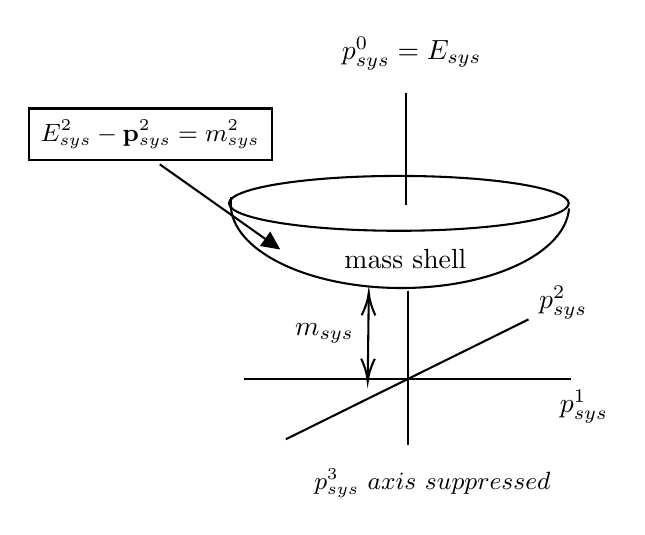
\begin{tikzpicture}[x=0.75pt,y=0.75pt,yscale=-1,xscale=1]
%uncomment if require: \path (0,300); %set diagram left start at 0, and has height of 300

%Shape: Ellipse [id:dp5571456664169634] 
\draw   (405,104.58) .. controls (405,97.28) and (441.64,91.37) .. (486.83,91.37) .. controls (532.03,91.37) and (568.67,97.28) .. (568.67,104.58) .. controls (568.67,111.88) and (532.03,117.8) .. (486.83,117.8) .. controls (441.64,117.8) and (405,111.88) .. (405,104.58) -- cycle ;
%Shape: Arc [id:dp5755134037737296] 
\draw  [draw opacity=0] (568.82,107.06) .. controls (567.12,128.58) and (531.16,145.6) .. (487.13,145.37) .. controls (442.1,145.14) and (405.69,126.94) .. (405.81,104.73) .. controls (405.81,103.68) and (405.9,102.64) .. (406.06,101.61) -- (487.34,105.16) -- cycle ; \draw   (568.82,107.06) .. controls (567.12,128.58) and (531.16,145.6) .. (487.13,145.37) .. controls (442.1,145.14) and (405.69,126.94) .. (405.81,104.73) .. controls (405.81,103.68) and (405.9,102.64) .. (406.06,101.61) ;
%Straight Lines [id:da112253833250195] 
\draw    (490.34,51.59) -- (490.34,105.16) ;
%Straight Lines [id:da11852275241679622] 
\draw    (491.34,146.59) -- (491.34,220.8) ;
%Straight Lines [id:da8670761805887259] 
\draw    (412,189.37) -- (569.67,189.37) ;
%Straight Lines [id:da3801545380094623] 
\draw    (432.38,218.24) -- (549.29,160.5) ;
%Straight Lines [id:da8071395461508041] 
\draw    (471.86,188.37) -- (472.32,149.59) ;
\draw [shift={(472.34,147.59)}, rotate = 450.68] [color={rgb, 255:red, 0; green, 0; blue, 0 }  ][line width=0.75]    (10.93,-3.29) .. controls (6.95,-1.4) and (3.31,-0.3) .. (0,0) .. controls (3.31,0.3) and (6.95,1.4) .. (10.93,3.29)   ;
\draw [shift={(471.83,190.37)}, rotate = 270.68] [color={rgb, 255:red, 0; green, 0; blue, 0 }  ][line width=0.75]    (10.93,-3.29) .. controls (6.95,-1.4) and (3.31,-0.3) .. (0,0) .. controls (3.31,0.3) and (6.95,1.4) .. (10.93,3.29)   ;
%Straight Lines [id:da37867462769054516] 
\draw    (371.67,85.8) -- (427.22,125.07) ;
\draw [shift={(429.67,126.8)}, rotate = 215.26] [fill={rgb, 255:red, 0; green, 0; blue, 0 }  ][line width=0.08]  [draw opacity=0] (8.93,-4.29) -- (0,0) -- (8.93,4.29) -- cycle    ;

% Text Node
\draw (451,167.37) node    {$m_{sys}$};
% Text Node
\draw (490,131.37) node   [align=left] {mass shell};
% Text Node
\draw (576,202.37) node    {$p^{1}_{sys}$};
% Text Node
\draw (566,152.37) node    {$p^{2}_{sys}$};
% Text Node
\draw (493,32.37) node    {$p^{0}_{sys} =E_{sys}$};
% Text Node
\draw    (308.5,58.87) -- (425.5,58.87) -- (425.5,83.87) -- (308.5,83.87) -- cycle  ;
\draw (367,71.37) node  [font=\small]  {$E^{2}_{sys} -\mathbf{p}^{2}_{sys} =m^{2}_{sys}$};
% Text Node
\draw (503,239.37) node  [font=\small]  {$p^{3}_{sys} \ axis\ suppressed$};


\end{tikzpicture}

\end{center}
The schematic above shows the following relation:(i.e. a shell upon which real particle energies and 3-momenta values must lie.)
\begin{equation}
E_{s y s}^{2}-\mathbf{p}_{s y s}^{2}=m_{s y s}^{2}
\end{equation}
For a system of particles, we determine an invariant mass $m_{sys}$. The surface in the figure is called the \textbf{mass shell}. Real particles must be "on the mass shell". Virtual particles can be, and generally are "off shell". $m_{sys}=0$ for photons, so the photon mass shell touches the origin.

From the delta function in (\ref{S-1-fi}), we know that the outgoing 4-momentum for the photon of Fig(\ref{fig:single-vertex}) equals the incoming total 4-momentum of the electron and positron:
$$
p_{i}^{\mu}=\left(\begin{array}{l}
{E_{1}+E_{2}} \\
{\mathbf{p}_{1}+\mathbf{p}_{2}}
\end{array}\right)=p_{f}^{\mu}=\left(\begin{array}{c}
{\omega_{k_{1}}} \\
{\mathbf{k}_{1}}
\end{array}\right)
$$
For initial state
$$
p_{i}^{\mu} p_{i \mu}=\left(E_{1}+E_{2}\right)^{2}-\left(\mathbf{p}_{1}+\mathbf{p}_{2}\right) \cdot\left(\mathbf{p}_{1}+\mathbf{p}_{2}\right)=m_{s y s}^{2} \neq 0
$$
For final state
$$
p_{f}^{\mu} p_{f \mu}=\underbrace{\left(E_{1}+E_{2}\right)^{2}}_{\omega_{\mathrm{k}_{1}}}-\underbrace{\left(\mathrm{p}_{1}+\mathrm{p}_{2}\right)}_{\mathrm{k}_{1}} \cdot \underbrace{\left(\mathrm{p}_{1}+\mathrm{p}_{2}\right)}_{\mathrm{k}_{1}}=m_{\mathrm{sys}}^{2} \neq 0
$$
\textbf{which must equal zero for a photon. That it doesn't equal zero means we can't produce a real photon.}
\begin{qt}
    $$
S_{f i}=\left\langle\gamma\left|S_{1}^{(1)} +\underbrace{S_{2}^{(1)}+\ldots+S_{8}^{(1)}}_{\text {all yield zero }}\right| e_{\mathbf{p}_{1}, n}^{-}, e_{\mathbf{p}_{2}, r_{2}}^{+}\right\rangle=\underbrace{\langle\gamma|}_{\text {on-shell }} \underbrace{\left.S_{1}^{(1)} | e_{p_{1}, n}^{-}, e^{+}_{\mathrm{p}_{2}, r_{2}}\right\rangle}_{\text {off-shell photon }}=0
$$
because the only ket left is an off-shell photon with $k^{\mu}=p_{1}^{\mu}+p_{2}^{\mu},$ and that is a different state from, and thus orthogonal to, any real final state photon, which cannot have this value for $k^{\mu} .$ Thus, the transition amplitude for Fig. (\ref{fig:single-vertex}) is zero. Similar logic for all single vertex interactions means we can simply ignore $S^{(1)}$ from here on.
\end{qt}
\section{Physical Meaning of S(2)}
\textbf{$S^{(2)}$ will represent two vertex interactions.} The first term of $S^{(2)}$ is $S_A^{(2)}$:
$$
S_{A}^{(2)}=-\frac{1}{2 !} e^{2} \iint d^{4} x_{1} d^{4} x_{2} N\left\{(\bar{\psi} \cancel{A} \psi)_{x_{1}}(\bar{\psi} \cancel{A} \psi)_{x_{2}}\right\}
$$
\textbf{\redp{This represents two independent processes like $S^{(1)}$.}} The two processes
do not interact with one another and each behaves as if the other did not exist. There is no virtual particle (Feynman propagator) linking them. Think of two separate single vertex Feynman diagrams. Neither of these can occur, so $S_A^{(2)}$ does not represent a real physical process and is ignored in QFT.

\subsection{The photon propagator term}
Consider the second term of $S^{(2)}$ acting on an initial state
\begin{equation}
S_{B}^{(2)}|i\rangle=-\frac{1}{2 !} e^{2} \iint d^{4} x_{1} d^{4} x_{2} N\left\{(\bar{\psi} \linktwoterms{\cancel{A}}{\psi)_{x_{1}}(\bar{\psi}}{\cancel{A}} \psi)_{x_{2}}\right\}|i\rangle
\label{four-external-lepton-interactions}
\end{equation}
The only initial states (\ref{four-external-lepton-interactions}) could destroy would be electron/positron states; and the only final states it could create would be electron/positron states. \textbf{We call these types of interactions four external lepton interactions.}
\begin{figure}[H]
    \centering
\tikzset{every picture/.style={line width=0.75pt}} %set default line width to 0.75pt        
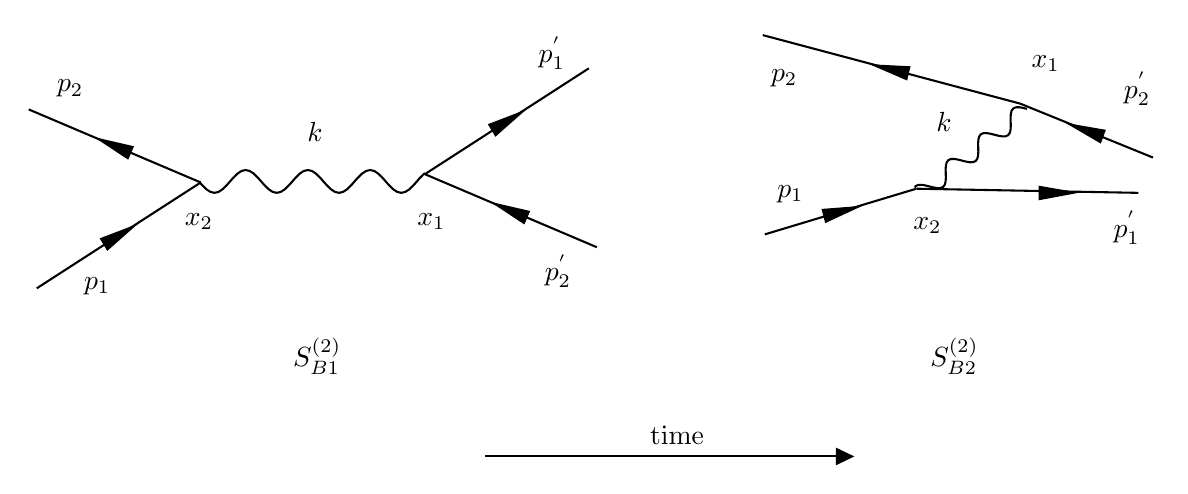
\begin{tikzpicture}[x=0.75pt,y=0.75pt,yscale=-1,xscale=1]
%uncomment if require: \path (0,300); %set diagram left start at 0, and has height of 300

%Straight Lines [id:da29515338597014595] 
\draw    (39,63) -- (121.87,98.2) ;
%Straight Lines [id:da8356384809428652] 
\draw    (121.87,98.2) -- (42.87,149.2) ;
%Shape: Wave [id:dp48547110897765466] 
\draw   (121,97.7) .. controls (123.45,100.52) and (125.79,103.2) .. (128.5,103.2) .. controls (131.21,103.2) and (133.55,100.52) .. (136,97.7) .. controls (138.45,94.88) and (140.79,92.2) .. (143.5,92.2) .. controls (146.21,92.2) and (148.55,94.88) .. (151,97.7) .. controls (153.45,100.52) and (155.79,103.2) .. (158.5,103.2) .. controls (161.21,103.2) and (163.55,100.52) .. (166,97.7) .. controls (168.45,94.88) and (170.79,92.2) .. (173.5,92.2) .. controls (176.21,92.2) and (178.55,94.88) .. (181,97.7) .. controls (183.45,100.52) and (185.79,103.2) .. (188.5,103.2) .. controls (191.21,103.2) and (193.55,100.52) .. (196,97.7) .. controls (198.45,94.88) and (200.79,92.2) .. (203.5,92.2) .. controls (206.21,92.2) and (208.55,94.88) .. (211,97.7) .. controls (213.45,100.52) and (215.79,103.2) .. (218.5,103.2) .. controls (221.21,103.2) and (223.55,100.52) .. (226,97.7) .. controls (227.29,96.21) and (228.56,94.75) .. (229.87,93.72) ;
%Straight Lines [id:da12560516877601058] 
\draw    (308.87,43.2) -- (229.87,94.2) ;
%Straight Lines [id:da6163580842382406] 
\draw    (229.87,94.2) -- (312.73,129.4) ;
%Shape: Triangle [id:dp685466344952348] 
\draw  [fill={rgb, 255:red, 0; green, 0; blue, 0 }  ,fill opacity=1 ] (72.99,77.4) -- (89.03,81.1) -- (86.72,86.49) -- cycle ;
%Shape: Triangle [id:dp005741777290943051] 
\draw  [fill={rgb, 255:red, 0; green, 0; blue, 0 }  ,fill opacity=1 ] (263.86,108.6) -- (279.9,112.3) -- (277.58,117.69) -- cycle ;
%Shape: Triangle [id:dp11625025303653935] 
\draw  [fill={rgb, 255:red, 0; green, 0; blue, 0 }  ,fill opacity=1 ] (89.3,119.51) -- (76.95,130.4) -- (73.92,125.38) -- cycle ;
%Shape: Triangle [id:dp30589288901509604] 
\draw  [fill={rgb, 255:red, 0; green, 0; blue, 0 }  ,fill opacity=1 ] (276.3,64.51) -- (263.95,75.4) -- (260.92,70.38) -- cycle ;
%Straight Lines [id:da5797267371251957] 
\draw    (392.67,27.2) -- (516.67,60.2) ;
%Straight Lines [id:da5534129518575254] 
\draw    (516.67,60.2) -- (580.67,86.2) ;
%Straight Lines [id:da13099665104403413] 
\draw    (393.67,123.2) -- (466.67,101.2) ;
%Straight Lines [id:da23142398769308015] 
\draw    (466.67,101.2) -- (573.67,103.2) ;
%Shape: Triangle [id:dp9580604600019759] 
\draw  [fill={rgb, 255:red, 0; green, 0; blue, 0 }  ,fill opacity=1 ] (438,110.15) -- (423.07,117.08) -- (421.59,111.41) -- cycle ;
%Shape: Triangle [id:dp6776790710702215] 
\draw  [fill={rgb, 255:red, 0; green, 0; blue, 0 }  ,fill opacity=1 ] (542.27,103.15) -- (526.08,106.18) -- (526.05,100.32) -- cycle ;
%Shape: Wave [id:dp647042217139919] 
\draw   (519.94,62.74) .. controls (517.3,62.05) and (514.78,61.39) .. (513.37,62.52) .. controls (511.95,63.64) and (512.03,66.24) .. (512.11,68.97) .. controls (512.2,71.7) and (512.28,74.3) .. (510.86,75.42) .. controls (509.45,76.55) and (506.93,75.89) .. (504.29,75.2) .. controls (501.65,74.51) and (499.14,73.85) .. (497.72,74.98) .. controls (496.3,76.1) and (496.38,78.7) .. (496.47,81.43) .. controls (496.55,84.16) and (496.63,86.76) .. (495.22,87.88) .. controls (493.8,89.01) and (491.28,88.35) .. (488.64,87.66) .. controls (486.01,86.96) and (483.49,86.31) .. (482.07,87.43) .. controls (480.66,88.56) and (480.74,91.16) .. (480.82,93.89) .. controls (480.91,96.61) and (480.98,99.21) .. (479.57,100.34) .. controls (478.15,101.47) and (475.64,100.81) .. (473,100.12) .. controls (470.36,99.42) and (467.84,98.77) .. (466.43,99.89) .. controls (466.19,100.08) and (466,100.31) .. (465.84,100.58) ;
%Shape: Triangle [id:dp3657896804062972] 
\draw  [fill={rgb, 255:red, 0; green, 0; blue, 0 }  ,fill opacity=1 ] (446.78,41.87) -- (463.22,42.67) -- (461.89,48.39) -- cycle ;
%Shape: Triangle [id:dp26512090066334226] 
\draw  [fill={rgb, 255:red, 0; green, 0; blue, 0 }  ,fill opacity=1 ] (541.06,70.42) -- (557.28,73.22) -- (555.27,78.73) -- cycle ;
%Straight Lines [id:da8555170327907058] 
\draw    (258.77,230.2) -- (433.77,230.2) ;
\draw [shift={(436.77,230.2)}, rotate = 180] [fill={rgb, 255:red, 0; green, 0; blue, 0 }  ][line width=0.08]  [draw opacity=0] (8.93,-4.29) -- (0,0) -- (8.93,4.29) -- cycle    ;

% Text Node
\draw (59,53) node    {$p_{2}$};
% Text Node
\draw (72,148) node    {$p_{1}$};
% Text Node
\draw (291,36) node    {$p^{'}_{1}$};
% Text Node
\draw (294,141) node    {$p^{'}_{2}$};
% Text Node
\draw (121,117) node    {$x_{2}$};
% Text Node
\draw (233,117) node    {$x_{1}$};
% Text Node
\draw (177,74) node    {$k$};
% Text Node
\draw (529,41) node    {$x_{1}$};
% Text Node
\draw (472,119) node    {$x_{2}$};
% Text Node
\draw (573,53) node    {$p^{'}_{2}$};
% Text Node
\draw (568,120) node    {$p^{'}_{1}$};
% Text Node
\draw (480,69) node    {$k$};
% Text Node
\draw (406,104) node    {$p_{1}$};
% Text Node
\draw (403,48) node    {$p_{2}$};
% Text Node
\draw (178,182) node    {$S^{( 2)}_{B1}$};
% Text Node
\draw (485,182) node    {$S^{( 2)}_{B2}$};
% Text Node
\draw (351.33,220) node   [align=left] {time};


\end{tikzpicture}

    \caption{Bhabha scattering can occur in two ways}
    \label{fig:Bhabha-scattering}
\end{figure}
In Fig.(\ref{fig:Bhabha-scattering}), both scenarios have the same incoming and outgoing particle states, which are all that we can measure. The internal virtual particle interaction is not measurable so there is no way
we can tell which of the two interactions gave us the Bhabha scattering.Bhabha scattering actually entails both types of interaction, \bluep{i) an annihilation of $e^{-}$ with an $e^{+}$ followed by a creation of the same two types of particles,  and ii) one of the incoming particles emitting a virtual photon which is then absorbed by the other particle. i.e., the same incoming momenta and spins for both and the same outgoing momenta and spins for both.}

\subsubsection{First type of Bhabha Scattering}
Consider the first type of Bhabha scattering with the S operator acting on the incoming state,
\begin{equation}
S_{B}^{(2)}\left|e_{\mathrm{p}_{1}, \mathrm{r_1}}^{-}, e_{\mathrm{p}_{2}, \mathrm{r}_{2}}^{+}\right\rangle=-\frac{1}{2 !} e^{2} \iint d^{4} x_{1} d^{4} x_{2} N\left\{(\bar{\psi} \linktwoterms{\cancel{A}}{ \psi)_{x_{1}}(\bar{\psi}}{\cancel{A}}  \psi)_{x_{2}}\right\}\left|e_{\mathrm{p}_1, \mathrm{r}_1}^{-}, e^{+}_{\mathrm{p}_{2}, r_{2}}\right\rangle
\end{equation}
At $x_{2},$ the $\psi^{+}$ part of $\psi_{x_{2}}$ would destroy the ket electron; the $\bar{\psi}^+$ part of $\bar{\psi}_{x_{2}}$ would destroy the ket positron; and we would be left with the vacuum $|0\rangle$. The propagator would then create a virtual photon at $x_{2}$ and propagate it to $x_{1}$ where it would be destroyed. Then, the $\psi^{-}$ part of $\psi_{x_{1}}$ would create a positron at $x_{1} ;$ and the $\bar{\psi}$ part of $\bar{\psi}_{x_{1}}$ would create an electron there.
$$
S_{B 1}^{(2)}=\frac{-e^{2}}{2}\left\langle e^-_{p_{1}^{\prime}, r^{\prime}_1}, e^{+}_{ p_{2^{\prime}} r_{2}^{\prime}}\right|\iint d^{4} x_{1} d^{4} x_{2}\left((\bar{\psi}^{-} \linktwoterms{\cancel{A}}{ \psi^{-})_{x_{1}}(\bar{\psi}^{+}}{\cancel{A}} \psi^{+})_{x_{2}}+\right.
$$
$$
\left.N\left\{(\bar{\psi}^{+} \linktwoterms{\cancel{A}}{ \psi^{+})_{x_{1}}(\bar{\psi}^-}{\cancel{A}} \psi^{-})_{x_{2}}\right\}\right) \left| e_{\mathfrak{p}_{1}, r_{1}}^{-}, e^{+}_{\mathfrak{p}_{2}, r_{2}}\right\rangle
$$
in which we can think of the second term above as annihilation at $x_{1}$ and creation at $x_{2}$ instead of the other way around. When we normal order the second term, $\psi^{+}\left(x_{1}\right)$ is switched once with $\bar{\psi}^-$ ( $x_{2}$ ) introducing a minus sign, then switch order with $\psi^{-}\left(x_{2}\right),$ introducing a second minus sign and resulting in no total sign change. The propagator is just a number, so it can be moved anywhere without effect (though care
has to be taken with keeping the correct spinor multiplication order).

Carrying out similar switching for $\bar{\psi}^{+}\left(x_{1}\right)$ with $\bar{\psi}^{-}\left(x_{2}\right)$ and then $\psi^{-}\left(x_{2}\right),$ we end up with
$$
S_{B 1}^{(2)}=\frac{-e^{2}}{2}\left\langle e_{p_{1}^{\prime}, r^{\prime}_1}^-, e^{+}_{p_{2}^{\prime}, r_{2}^{\prime}}\right| \iint d^{4} x_{1} d^{4} x_{2}\left((\bar{\psi}^{-} \linktwoterms{\cancel{A}}{ \psi^{-})_{x_{1}}(\bar{\psi}^{+} }{\cancel{A}} \psi^{+})_{x_{2}}\right.+\left.(\bar{\psi}^{-} \linktwoterms{\cancel{A}}{ \psi^{-})_{x_{2}}(\bar{\psi}^{+}}{\cancel{A}} \psi^{+})_{x_{1}}\right)|\left.e_{p_{1}, r_1}^{-}, e^{+}_{p_{2}, r_{2}}\right\rangle
$$
$$
=-e^{2}\left\langle e_{p_{1}^{\prime}, r_1^{\prime}}^{-}, e^{+}_{p_{2}^{\prime}, r_{2}^{\prime}}\right| \iint d^{4} x_{1} d^{4} x_{2}(\bar{\psi}^{-} \linktwoterms{\cancel{A}}{ \psi^{-})_{x_{1}}(\bar{\psi}^{+}}{\cancel{A}} \psi^{+})_{x_{2}}\left|e_{\mathfrak{p}_{1}, r_1}^{-}, e_{p_{2}, r_{2}}^{+}\right\rangle
$$
\redp{where in second line we simply exchanged dummy variables in the second term of the first line to get the second line}. Substituting the field equation solutions for the operators at $x_2$ above, we have
$$
S_{B 1}^{(2)}=-e^{2}\left\langle e_{\mathrm{p}_{1}^{\prime}, r_1^{\prime}}^-, e_{\mathrm{p}_{2}^{\prime}, r_{2}}^{+}\right| \iint d^{4} x_{1} d^{4} x_{2}\left(\bar{\psi}^{-} \gamma^{\mu} \psi^{-}\right)_{x_{1}} i D_{F \mu \nu}\left(x_{1}-x_{2}\right) \times
$$
$$
\left(\sum_{r^{\prime}, p^{\prime}} \sqrt{\frac{m}{V E_{p'}}} d _{r'}\left(p^{\prime}\right) \bar{v}_{r^{\prime}}\left(p^{\prime}\right) e^{-i p^{\prime} x_{2}}\right) \gamma^{v}\left(\sum_{r^{\prime\prime} p^{\prime\prime}}, \sqrt{\frac{m}{V E_{p^{\prime\prime}}}} c_{r^{\prime\prime}}\left(\mathbf{p}^{\prime\prime}\right) u_{r^{\prime\prime}}\left(\mathbf{p}^{\prime \prime}\right) e^{-i p^{\prime\prime} \mathbf{x}_{2}}\right)\left|e_{\mathfrak{p}_{1}, r_{1}}^{-}, e^{+}_{\mathfrak{p}_{2}, r_{2}}\right\rangle
$$
The terms do match up turn the ket into the vacuum. So the equation above becomes
$$
S_{B 1}^{(2)}=-e^{2}\left\langle e^-_{\mathrm{p}_1^{\prime}, r_1^{\prime}}, e^{+}_{\mathrm{p}_{2}^{\prime}, r_{2}^{\prime}}\right| \iint d^{4} x_{1} d^{4} x_{2}\left(\bar{\psi}^{-} \gamma^{\mu} \psi^{-}\right)_{x_{1}} i D_{F \mu \nu}\left(x_{1}-x_{2}\right)\times
$$
$$
\frac{m}{V} \sqrt{\frac{1}{E_{\mathrm{p}_{1}} E_{\mathrm{p}_{2}}}} \bar{v}_{r_{2}}\left(\mathrm{p}_{2}\right) \gamma^{\nu} u_{r_{1}}\left(\mathrm{p}_{1}\right) e^{-i p_{2} x_{2}} e^{-i p_{1} x_{2}}|0\rangle
$$
Substituting the propagator relation we derived at the end of Chap 4 and rearranging,
$$
S_{B 1}^{(2)}=-e^{2}\left(e_{\mathrm{p}^{\prime} \mathrm{i}, \mathrm{r}^{\prime}}, e_{\mathrm{p}_{2}^{\prime}, \mathrm{r}_{2}^{\prime}}^{+} | \int\left(\bar{\psi}^{-} \gamma^{\mu} \psi^{-}\right)_{x_{1}} \times\right.\left(\int\left(\frac{-i g_{\mu \nu}}{(2 \pi)^{4}} \int \frac{e^{-i k\left(x_{1}-x_{2}\right)}}{k^{2}+i \varepsilon} d^{4} k\right) \frac{m}{V}\right.
$$
$$
\left.\sqrt{\frac{1}{E_{\mathrm{p}_{1}} E_{\mathrm{p}_{2}}}} \bar{v}_{r_{2}}\left(\mathrm{p}_{2}\right) \gamma^{v} u_{r_{1}}\left(\mathbf{p}_{1}\right) e^{-i p_{2} x_{2}} e^{-i p_{1} x_{2}} d^{4} x_{2}\right) d^{4} x_{1}|0\rangle
$$
$$
=e^{2}\left\langle e^-_{\mathrm{p}_{1}^{\prime}, r_{1}^{\prime}}, e_{\mathrm{p}_{2}^{\prime}, r_{2}^{\prime}}^{+}\right| \int\left(\bar{\psi}^- \gamma^{\mu} \psi^{-}\right)_{x_{1}} i g_{\mu \nu} \bar{v}_{r_{2}}\left(\mathbf{p}_{2}\right) \gamma^{\nu} u_{r_{1}}\left(\mathbf{p}_{1}\right) \times
$$
$$
\frac{m}{V} \sqrt{\frac{1}{E_{p_{1}} E_{p_{2}}}}\left(\int \frac{1}{k^{2}+i \varepsilon} e^{-i k x_{1}} \frac{1}{(2 \pi)^{4}}\underbrace{\left(\int e^{i k x_{2}} e^{-i p_{2} x_{2}} e^{-i p_{1} x_{2}} d^{4} x_{2}\right)}_{(2 \pi)^{4} \delta^{(4)}\left(k-p_{2}-p_{1}\right)} d^{4} k\right) d^{4} x_{1}|0\rangle
$$
\redp{The delta relation that results above tells us that $k=p_1+p_2$, the virtual photon 4-momentum equals th sum of the incoming particles 4-momenta. Again, we see conservation of energy and 3-momentum at a vertex.} \textbf{And again, we see that the photon particle is off-shell, i.e.,$k_{\mu}k^{\mu}=m^2_{sys}\neq0$.}

The delta relation picks the single value $k=p_1+p_2$ out of the integration over $k$. So now,
$$
S_{B 1}^{(2)}=e^{2}\left\langle e_{\mathrm{p}_{1}^{\prime}, r_{1}^{\prime}}^{-}, e_{\mathrm{p}_{2}^{\prime}, \mathrm{r}_{2}^{\prime}}^{+}\right| \frac{m}{V}\sqrt{\frac{1}{E_{\mathrm{p}_{1}} E_{\mathrm{p}_{2}}}}\left(\int\left(\bar{\psi}^- \gamma^{\mu} \psi^{-}\right)_{x_{1}} \frac{e^{-i\left(p_{2}+p_{1}\right) x_{1}}}{\left(p_{2}+p_{1}\right)^{2}+i \varepsilon} d^{4} x_{1}\right)\times$$
$$ i g_{\mu \nu}\bar{v}_{r_{2}}\left(\mathbf{p}_{2}\right) \gamma^{\nu} u_{r_{1}}\left(\mathbf{p}_{1}\right)|0\rangle
$$
Substituting the relations for the spinor creation field operators at $x_1$ yields
$$
S_{B 1}^{(2)}=e^{2}\left(\frac{m}{V}\right)^{2} \sqrt{\frac{1}{E_{\mathrm{p}_{1}} E_{\mathrm{p}_{2}}}} \sqrt{\frac{1}{E_{\mathrm{p}^{\prime}_{1}} E_{\mathrm{p}^{\prime}_{2}}}}\left\langle e_{\mathrm{p}_{1}^{\prime}, r_1^{\prime}}^{-}, e_{\mathrm{p}_{2}^{\prime}, \mathrm{r}_{2}^{\prime}}^{+}\right|\left(\int e^{-i\left(p_{2}+p_{1}\right) x_{1}} e^{i\left(p_{1}^{\prime}+p_{2}^{\prime}\right) x_{1}} d^{4} x_{1}\right) \times
$$
$$
\bar{u}_{r_{1}^{\prime}}\left(\mathbf{p}_{1}^{\prime}\right) \gamma^{\mu} v_{r_{2}^{\prime}}\left(\mathbf{p}_{2}^{\prime}\right) \frac{i g_{\mu v}}{\left(p_{2}+p_{1}\right)^{2}+i \varepsilon} \bar{v}_{r_{2}}\left(\mathbf{p}_{2}\right) \gamma^{v} u_{r_{1}}\left(\mathbf{p}_{1}\right)\left|e_{p_{1}^{\prime}, r_{1}^{\prime}}^-, e^{+}_{p_2^{\prime}, r_{2}^{\prime}}\right\rangle
$$
The integral over $x_{1}$ is another delta function telling us that $p_{2}^{\prime}+p^{\prime}_{1}=p_{2}+p_{1},$ the total outgoing $4$ -momentum equals the total incoming 4 -momentum, which, as we discovered earlier, equals the 4-momentum of the virtual photon propagator. Energy and 3 -momentum are conserved at every vertex. And the final, real particle state is on-shell.

The result of all this, where we note that the fraction factor in the equation above with the $i\varepsilon$ as part of the denominator is simply (up to a sign) the Feynman propagator in momentum space, is
\begin{qt}
    $$
\underbrace{S_{B 1}^{(2)}}_{\text { transition amplitude }}=\sqrt{\frac{m}{V E_{\mathrm{p}_1}}} \sqrt{\frac{m}{V E_{\mathrm{p}_2}}} \sqrt{\frac{m}{V E_{\mathrm{p}_1^{\prime}}}} \sqrt{\frac{m}{V E_{\mathrm{p}^{\prime}_{2}}}}(2 \pi)^{4} \delta^{(4)}\left(p_{1}+p_{2}-\left(p_{1}^{\prime}+p_{2}^{\prime}\right)\right)
$$
$$
\times \underbrace{\left(-e^{2}\right) \bar{u}_{r_{1}^{\prime}}\left(\mathbf{p}_{1}^{\prime}\right) \gamma^{\mu} v_{r_{2}^{\prime}}\left(\mathbf{p}_{2}^{\prime}\right) i D_{F \mu v}\left(k=p_{1}+p_{2}\right) \bar{v}_{r_{2}}\left(p_{2}\right) \gamma^{v} u_{r_{1}}\left(p_{1}\right)}_{\text {Feynman amplitude } \mathcal{M}_{B 1}^{(2)}}
$$
Note the definition of the Feynman amplitude for this interaction $\mathcal{M}_{B 1}^{(2)}$. Using that, we have
\begin{equation}
S_{B 1}^{(2)}=\left(\prod_{\mathbf{p}}^{\text {all ext fermions }} \sqrt{\frac{m}{V E_{\mathbf{p}}}}\right)(2 \pi)^{4} \delta^{(4)}\left(p_{1}+p_{2}-\left(p_{1}^{\prime}+p_{2}^{\prime}\right)\right) \mathcal{M}_{B 1}^{(2)}
\end{equation}
\end{qt}
\subsubsection{The second type of Bhabha scattering}
Note in Fig.(\ref{fig:Bhabha-scattering}), that on the RHS, either $x_2$ or $x_1$ could occur first, and our math takes care of both cases automatically. We start with the same fundamental relation we had for the first type of Bhabha scattering,
\begin{equation}
S_{B}^{(2)}\left|e_{\mathrm{p}_{1}, r_{1}}^{-}, e_{\mathrm{p}_{2}, r_{2}}^{+}\right\rangle=-\frac{e^{2}}{2!} \iint d^{4} x_{1} d^{4} x_{2} N\left\{(\bar{\psi} \linktwoterms{\cancel{A}}{ \psi)_{x_{1}}(\bar{\psi}}{\cancel{A} } \psi)_{x_{2}}\right\} \left| e_{\mathfrak{p}_{1},r_1}^-, e_{\mathrm{p}_{2}, \mathrm{r}_{2}}^{+}\right\rangle
\end{equation}
\textbf{\bluep{but this time, we pick the creation and destruction operators corresponding to the second type of
Bhabha scattering. That is, we have}}
$$
S^{(2)}_{B2}=\frac{-e^{2}}{2}\left\langle e^-_{p_{1}^{\prime}, r_{1}^{\prime}}, e^+_{p_{2}^{\prime}, r_{2}^{\prime}}\right| \times
$$
$$
\iint d^{4} x_{1} d^{4} x_{2} N\left\{(\bar{\psi}^{+} \linktwoterms{A_{\mu}}{ \gamma^{\mu} \psi^{-})_{x_{1}}(\bar{\psi}^{-}}{A_{v}} \gamma^{v} \psi^{+})_{x_{2}}+(\bar{\psi} \linktwoterms{A_{\mu}}{ \gamma^{\mu} \psi^{+})_{x_{1}}(\bar{\psi}^{+}}{ A_{v}} \gamma^{v} \psi^{-})_{x_{2}}\right\}\left|e_{\mathbf{p}_{1}, r_{1}}^{-}, e^{+}_{ \mathbf{p}_{2}, r_{2}}\right\rangle
$$
which, if \textbf{we switch dummy integration variables again, the first and second terms above are equivalent.} That eliminates the $1 / 2$ factor and leaves (where we now show spinor indices).
\begin{equation}
S_{B 2}^{(2)}=-e^{2}\langle e_{\mathrm{p}_{1}^{\prime}, r_{1}^{\prime}}^{-}, e^{+}_{\mathrm{p}_{2}^{\prime}, r_{2}^{\prime}}| \iint d^{4} x_{1} d^{4} x_{2} N \{(\bar{\psi}_{\alpha}^{+} \linktwoterms{A_{\mu}}{ \gamma_{\alpha \beta}^{\mu} \psi_{\beta}^{-})_{x_{1}}(\bar{\psi}_{\delta}^-}{ A_{\nu}} \gamma_{\delta \eta}^{\nu} \psi_{\eta}^{+})_{x_{2}}\} | e_{\mathrm{p}_{1}, r_{1}}^{-}, e_{\mathrm{p}_{2}, r_{2}}^{+}\rangle
\label{second-type-Bhabha}
\end{equation}
This can be visualized as the incoming electron destroyed at $x_{2}$ with the outgoing electron created a $x_{2}$ and a photon propagator starting at $x_{2}$. The incoming positron is destroyed at $x_{1}$ with the outgoing positron positron created at $x_{1}$ and the photon propagator ending at $x_{1}$. The reverse situation, where $x_{1}$ and $x_2$ are interchanged has been included by the factor of two enveloped.

Normal ordering (\ref{second-type-Bhabha}), where we now see the value of writing out spinor indices, give us
\begin{equation}
S_{B 2}^{(2)}=e^{2}\langle e_{p_{1}^{\prime}, r_1^{\prime}}^-, e^{+} _{p_2^{\prime}, r_{2}^{\prime}}| \iint d^{4} x_{1} d^{4} x_{2} (\bar{\psi}^{-}_{\delta})_{x_{2}}(\linktwoterms{A_{\mu}}{ \gamma_{\alpha \beta}^{\mu} \psi_{\beta}^{-})_{x_{1}}(\bar{\psi}_{\alpha}^{+})_{x_{1}}(}{A_{v}} \gamma_{\delta \eta}^{v} \psi_{\eta}^{+})_{x_{2}})|e_{p_{1}, r_1}^{-}, e^{+}_{p_{2}, r_{2}}\rangle
\label{second-type-Bhabha-scattering-2}
\end{equation}
Note carefully that we have to put (\ref{second-type-Bhabha-scattering-2}) not simply in any normal order, but \textbf{in the same normal order as (\ref{second-type-Bhabha}). That is, both transition sub amplitudes must have, in order from the right side moving leftward, operators performing $e^-$ destruction, $e^+$ destruction, $e^-$ creation, and $e^+$ creation.} We carry out similar steps to get
$$
S_{B 2}^{(2)}=e^{2} \frac{m^{2}}{V^{2}} \sqrt{\frac{1}{E_{\mathrm{p} 1} E_{\mathrm{p}_{2}} E_{\mathrm{p}_1^{\prime}} E_{\mathrm{p}_{2}^{\prime}}}} \bar{v}_{r_{2}}\left(\mathrm{p}_{2}\right) \gamma^{\mu} v_{r_{2}^{\prime}}\left(\mathbf{p}_{2}^{\prime}\right) \bar{u}_{\mathrm{r}^{\prime}}\left(\mathbf{p}_{\mathrm{I}}^{\prime}\right) \gamma^{v} u_{\mathrm{r}_{1}}\left(\mathbf{p}_{1}\right) \times
$$
$$
\left(\frac{-i g_{\mu \nu}}{\left(p_{1}-p_{1}^{\prime}\right)^{2}+i \varepsilon}\right) \underbrace{\left(\int e^{-i\left(p_{1}-p_{1}^{\prime}\right) x_{1}} e^{i p_{2}^{\prime} x_{1}} e^{-i p_{2} x_{1}} d^{4} x_{1}\right)}_{(2 \pi)^{4} \delta^{(4)}\left(p_{1}+p_{2}-\left(p_{1}^{\prime}+p_{2}^{\prime}\right)\right)}
$$
And thus, finally,
\begin{qt}
    \begin{equation}
S_{B 2}^{(2)}=\left(\prod_{\mathbf{p}}^{\text {allext fermions }} \sqrt{\frac{m}{V E_{\mathrm{p}}}}\right)(2 \pi)^{4} \delta^{(4)}\left(p_{1}+p_{2}-\left(p_{1}^{\prime}+p_{2}^{\prime}\right)\right) \mathcal{M}_{B 2}^{(2)}
\end{equation}
where
$$
\mathcal{M}_{B 2}^{(2)}=e^{2} \bar{v}_{r_{2}}\left(\mathbf{p}_{2}\right) \gamma^{\mu} v_{r^{\prime}_{2}}\left(\mathbf{p}_{2}^{\prime}\right) i D_{\mu v}\left(p_{2}^{\prime}-p_{2}\right) \bar{u}_{r_1^{\prime}}\left(\mathbf{p}_{1}^{\prime}\right) \gamma^{v} u_{r_1}\left(\mathbf{p}_{1}\right)
$$
\end{qt}
The total transition amplitude for 2nd order (n=2) Bhabha scatering is
\begin{equation}
S_{B h a b b a}=S_{B 1}^{(2)}+S_{B 2}^{(2)}=\left(\prod_{\mathrm{p}}^{\text {all fermions }} \frac{m}{\sqrt{\frac{m}{V E_{\mathrm{p}}}}}\right)(2 \pi)^{4} \delta^{(4)}\left(p_{1}+p_{2}-\left(p_{1}^{\prime}+p_{2}^{\prime}\right)\right)\left(\mathcal{M}_{B 1}^{(2)}+\mathcal{M}_{B 2}^{(2)}\right)
\end{equation}

\subsection{Compton Scattering}
Consider the third and fourth terms in $S^{(2)}$, acting on an initial state
\begin{equation}
S_{C}^{(2)}|i\rangle=-\frac{1}{2 !} e^{2} \iint d^{4} x_{1} d^{4} x_{2}(N\{(\bar{\psi} \linktwoterms{\cancel{A}}{ \psi)_{x_{1}}(\bar{\psi}}{\cancel{A}} \psi)_{x_{2}}\}+N\{(\bar{\psi}\linktwoterms{\cancel{A}}{ \psi)_{x_{1}}(\bar{\psi}}{\cancel{A}} \psi)_{x_{2}}\}) | i\rangle
\label{compton-scattering}
\end{equation}
The first term in (\ref{compton-scattering}) actually equals the second term as we can see from the following Box, and thus we can re-express (\ref{compton-scattering}) as
\begin{equation}
S_{C}^{(2)}|i\rangle=-\frac{1}{2 !} e^{2} \iint d^{4} x_{1} d^{4} x_{2}N\{(\bar{\psi}\linktwoterms{\cancel{A}}{ \psi)_{x_{1}}(\bar{\psi}}{\cancel{A}} \psi)_{x_{2}}\} | i\rangle
\label{compton-scattering-2}
\end{equation}
The contraction here is a fermion propagator and the incoming particles that could be destroyed by (\ref{compton-scattering-2}) could comprise an electron and a photon. Effectively, the electron and photon could scatter off one another as in Fig. (\ref{fig:compton-scattering}). This is called\textbf{ Compton scattering}. Note from Fig. (\ref{fig:compton-scattering}) than occur in two different ways, i.e., have the same real particles in and out.
\begin{figure}[H]
    \centering

\tikzset{every picture/.style={line width=0.75pt}} %set default line width to 0.75pt        

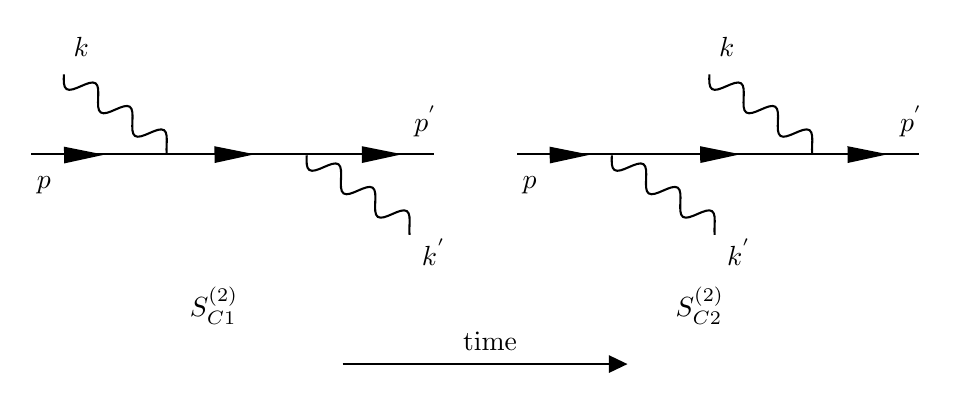
\begin{tikzpicture}[x=0.75pt,y=0.75pt,yscale=-1,xscale=1]
%uncomment if require: \path (0,300); %set diagram left start at 0, and has height of 300

%Straight Lines [id:da9652866719093866] 
\draw    (42,138.93) -- (235.87,138.93) ;
%Shape: Wave [id:dp4726907497917253] 
\draw   (57.65,100.38) .. controls (57.52,103.46) and (57.41,106.39) .. (58.9,107.41) .. controls (60.39,108.44) and (63.08,107.27) .. (65.9,106.03) .. controls (68.72,104.8) and (71.42,103.63) .. (72.91,104.65) .. controls (74.4,105.68) and (74.28,108.61) .. (74.16,111.68) .. controls (74.03,114.76) and (73.91,117.69) .. (75.4,118.71) .. controls (76.9,119.73) and (79.59,118.57) .. (82.41,117.33) .. controls (85.23,116.1) and (87.92,114.93) .. (89.41,115.95) .. controls (90.9,116.98) and (90.79,119.91) .. (90.66,122.98) .. controls (90.53,126.06) and (90.41,128.99) .. (91.9,130.01) .. controls (93.4,131.03) and (96.09,129.86) .. (98.91,128.63) .. controls (101.73,127.4) and (104.42,126.23) .. (105.91,127.25) .. controls (107.41,128.27) and (107.29,131.21) .. (107.16,134.28) .. controls (107.09,135.86) and (107.03,137.39) .. (107.19,138.65) ;
%Shape: Wave [id:dp581219954893428] 
\draw   (174.65,139.38) .. controls (174.52,142.46) and (174.41,145.39) .. (175.9,146.41) .. controls (177.39,147.44) and (180.08,146.27) .. (182.9,145.03) .. controls (185.72,143.8) and (188.42,142.63) .. (189.91,143.65) .. controls (191.4,144.68) and (191.28,147.61) .. (191.16,150.68) .. controls (191.03,153.76) and (190.91,156.69) .. (192.4,157.71) .. controls (193.9,158.73) and (196.59,157.57) .. (199.41,156.33) .. controls (202.23,155.1) and (204.92,153.93) .. (206.41,154.95) .. controls (207.9,155.98) and (207.79,158.91) .. (207.66,161.98) .. controls (207.53,165.06) and (207.41,167.99) .. (208.9,169.01) .. controls (210.4,170.03) and (213.09,168.86) .. (215.91,167.63) .. controls (218.73,166.4) and (221.42,165.23) .. (222.91,166.25) .. controls (224.41,167.27) and (224.29,170.21) .. (224.16,173.28) .. controls (224.09,174.86) and (224.03,176.39) .. (224.19,177.65) ;
%Shape: Triangle [id:dp4781339171474417] 
\draw  [fill={rgb, 255:red, 0; green, 0; blue, 0 }  ,fill opacity=1 ] (74.65,139.08) -- (58.25,142.65) -- (58.19,135.79) -- cycle ;
%Shape: Triangle [id:dp052309184229321404] 
\draw  [fill={rgb, 255:red, 0; green, 0; blue, 0 }  ,fill opacity=1 ] (147.15,138.86) -- (130.75,142.44) -- (130.69,135.57) -- cycle ;
%Shape: Triangle [id:dp3157602553829544] 
\draw  [fill={rgb, 255:red, 0; green, 0; blue, 0 }  ,fill opacity=1 ] (218.15,138.86) -- (201.75,142.44) -- (201.69,135.57) -- cycle ;
%Straight Lines [id:da7163286367875737] 
\draw    (276,138.93) -- (469.87,138.93) ;
%Shape: Wave [id:dp35829325317941596] 
\draw   (368.65,100.38) .. controls (368.52,103.46) and (368.41,106.39) .. (369.9,107.41) .. controls (371.39,108.44) and (374.08,107.27) .. (376.9,106.03) .. controls (379.72,104.8) and (382.42,103.63) .. (383.91,104.65) .. controls (385.4,105.68) and (385.28,108.61) .. (385.16,111.68) .. controls (385.03,114.76) and (384.91,117.69) .. (386.4,118.71) .. controls (387.9,119.73) and (390.59,118.57) .. (393.41,117.33) .. controls (396.23,116.1) and (398.92,114.93) .. (400.41,115.95) .. controls (401.9,116.98) and (401.79,119.91) .. (401.66,122.98) .. controls (401.53,126.06) and (401.41,128.99) .. (402.9,130.01) .. controls (404.4,131.03) and (407.09,129.86) .. (409.91,128.63) .. controls (412.73,127.4) and (415.42,126.23) .. (416.91,127.25) .. controls (418.41,128.27) and (418.29,131.21) .. (418.16,134.28) .. controls (418.09,135.86) and (418.03,137.39) .. (418.19,138.65) ;
%Shape: Wave [id:dp7598034423297523] 
\draw   (321.65,139.38) .. controls (321.52,142.46) and (321.41,145.39) .. (322.9,146.41) .. controls (324.39,147.44) and (327.08,146.27) .. (329.9,145.03) .. controls (332.72,143.8) and (335.42,142.63) .. (336.91,143.65) .. controls (338.4,144.68) and (338.28,147.61) .. (338.16,150.68) .. controls (338.03,153.76) and (337.91,156.69) .. (339.4,157.71) .. controls (340.9,158.73) and (343.59,157.57) .. (346.41,156.33) .. controls (349.23,155.1) and (351.92,153.93) .. (353.41,154.95) .. controls (354.9,155.98) and (354.79,158.91) .. (354.66,161.98) .. controls (354.53,165.06) and (354.41,167.99) .. (355.9,169.01) .. controls (357.4,170.03) and (360.09,168.86) .. (362.91,167.63) .. controls (365.73,166.4) and (368.42,165.23) .. (369.91,166.25) .. controls (371.41,167.27) and (371.29,170.21) .. (371.16,173.28) .. controls (371.09,174.86) and (371.03,176.39) .. (371.19,177.65) ;
%Shape: Triangle [id:dp8027556070300854] 
\draw  [fill={rgb, 255:red, 0; green, 0; blue, 0 }  ,fill opacity=1 ] (308.65,139.08) -- (292.25,142.65) -- (292.19,135.79) -- cycle ;
%Shape: Triangle [id:dp27556888831393467] 
\draw  [fill={rgb, 255:red, 0; green, 0; blue, 0 }  ,fill opacity=1 ] (381.15,138.86) -- (364.75,142.44) -- (364.69,135.57) -- cycle ;
%Shape: Triangle [id:dp8251492979907598] 
\draw  [fill={rgb, 255:red, 0; green, 0; blue, 0 }  ,fill opacity=1 ] (452.15,138.86) -- (435.75,142.44) -- (435.69,135.57) -- cycle ;
%Straight Lines [id:da46165972339858774] 
\draw    (192,239.93) -- (326.17,239.93) ;
\draw [shift={(329.17,239.93)}, rotate = 180] [fill={rgb, 255:red, 0; green, 0; blue, 0 }  ][line width=0.08]  [draw opacity=0] (8.93,-4.29) -- (0,0) -- (8.93,4.29) -- cycle    ;

% Text Node
\draw (48,153.93) node    {$p$};
% Text Node
\draw (232,122.93) node    {$p^{'}$};
% Text Node
\draw (236,185.93) node    {$k^{'}$};
% Text Node
\draw (66,86.93) node    {$k$};
% Text Node
\draw (130,211.93) node    {$S^{( 2)}_{C1}$};
% Text Node
\draw (282,153.93) node    {$p$};
% Text Node
\draw (466,122.93) node    {$p^{'}$};
% Text Node
\draw (383,185.93) node    {$k^{'}$};
% Text Node
\draw (377,86.93) node    {$k$};
% Text Node
\draw (364,211.93) node    {$S^{( 2)}_{C2}$};
% Text Node
\draw (263,228.93) node   [align=left] {time};


\end{tikzpicture}

    \caption{Compton Scattering Can Occur in Two Ways}
    \label{fig:compton-scattering}
\end{figure}
The LH vertex on each side of Fig.(\ref{fig:compton-scattering}) with $x_2$, and the RH with $x_1$, as it would be easier to track the analysis. The interaction could occur in either of the ways we label above as $S_{C 1}^{(2)}$ or $S_{C 2}^{(2)} .$ That is, either i) an electron could absorb a photon (equivalent to an electron and a photon being destroyed and a virtual electron being created at $x_{2}$ ) and later emit a photon(equivalent to the virtual electron being destroyed and both a real electron and a real photon being created at $x_1$); or ii) an electron could emit a photon (equivalent to an electron being destroyed and a real photon along with a virtual electron being created at $x_2$), and later absorbed a photo (equivalent to the virtual electron and a real photon being destroyed while a real electron is create at $x_1$).

\redp{Note that only the $S_{C}^{(2)}$ terms of all the $n=2$ terms will result in destruction of an initial electron and photon ket. }The $S$ matrix transition amplitude for second order Compton scattering is thus (with incoming particles unprimed, outgoing primed)
\begin{equation}
S_{\text {Compton }}=\langle f|S| i\rangle=\left\langle e^-_{\mathbf{p}^{\prime}, s^{\prime}}, \gamma_{\mathbf{k}^{\prime} r^{\prime}}\left|\left(-e^{2}\right) \iint d^{4} x_{1} d^{4} x_{2} N \int\left((\vec{\psi} \linktwoterms{\cancel{A}}{ \psi)_{x_{1}}(\bar{\psi}}{\cancel{A}} \psi)_{x_{2}}\right)\right| e_{\mathbf{p}, s}^{-}, \gamma_{\mathbf{k}, r}\right\rangle
\end{equation}
\begin{equation}
=-e^{2}\left\langle e^-_{\mathbf{p}^{\prime} s^{\prime}}, \gamma_{\mathbf{k}^{\prime}, r^{\prime}}\right| \iint d^{4} x_{1} d^{4} x_{2} N\left\{\left(\bar{\psi}^{+}+\bar{\psi}^{-}\right)_{x_{1}}\left(\cancel{A}^{+}+\cancel{A}^{-}\right)_{x_{1}} \times\right.
\end{equation}
$$
\left.\left(i S_{F}\left(x_{1}-x_{2}\right)\right)\left(\cancel{A}^{+}+\cancel{A}^{-}\right)_{x_{2}}\left(\psi^{+}+\psi^{-}\right)_{x_{2}}\right\}\left|e_{\mathbf{p}, s}^{-}, \gamma_{\mathbf{k}, r}\right\rangle
$$
After the operators raise and lower the ket, only two terms in the equation above remain:
\begin{equation}
\begin{split}
S_{\text {Compton }}&=-e^{2}\left\langle e^-_{\mathbf{p}^{\prime}, s^{\prime}}, \gamma_{\mathbf{k}^{\prime}, r^{\prime}}\right| \iint d^{4} x_{1} d^{4} x_{2} \underbrace{N\left\{\bar{\psi}_{x_{1}}^{-} \cancel{A}_{x_{1}}^{-}\left(i S_{F}\left(x_{1}-x_{2}\right)\right) \cancel{A}_{x_{2}}^{+} \psi_{x_{2}}^{+}\right.}_
{S_{C 1}^{(2)} \text { term } }\\
&+\underbrace{\bar{\psi}_{x_{1}}^{-} \cancel{A}_{x_{1}}^{+}\left(i S_{F}\left(x_{1}-x_{2}\right)\right) \cancel{A}_{x_{2}}^{-} \psi_{x_{2}}^{+}}_{\text {will result in } S_{C_{2}}^{(2)} \text { term }}\}\left|e_{\mathbf{p}, s}^{-}, \gamma_{\mathbf{k}, r}\right\rangle
\end{split}
\end{equation}
\begin{qt}
    The full second order Compton transition amplitude, including both cases of Fig.(\ref{fig:compton-scattering}), is
    \begin{equation}
    \begin{split}
        S_{\text {Compton }}&=\left(\prod_{\mathbf{p}^{''}}^{\text {all fermions }} \sqrt{\frac{m}{V E_{\mathrm{p}^{''}}}}\right)\left(\prod_{\mathbf{p}^{''}}^{\text {all bosons }} \sqrt{\frac{1}{2 V \omega_{\mathbf{k}^{\prime\prime}}}}\right)(2 \pi)^{4}\times\\
        &\delta^{(4)}\left(p^{\prime}+k^{\prime}-p-k\right)\left(\mathcal{M}_{C 1}^{(2)}+\mathcal{M}_{C 2}^{(2)}\right)
    \end{split}
\end{equation}
where
$$
\mathcal{M}_{C 1}^{(2)}=-e^{2} \bar{u}_{s^{\prime}, \alpha}\left(\mathbf{p}^{\prime}\right) \varepsilon_{\mu, r^{\prime}}\left(\mathbf{k}^{\prime}\right) \gamma_{\alpha \beta}^{\mu} i S_{F \beta \delta}(q=p+k) \varepsilon_{\nu, r}(\mathbf{k}) \gamma_{\delta \eta}^{\nu} u_{s, \eta}(\mathbf{p})
$$
$$
\mathcal{M}_{C 2}^{(2)}=-e^{2} \bar{u}_{s^{\prime}, \alpha}\left(\mathbf{p}^{\prime}\right) \varepsilon_{\mu, r}(\mathbf{k}) \gamma_{\alpha \beta}^{\mu} i S_{F \beta \delta}\left(q=p-k^{\prime}\right) \varepsilon_{\nu, r^{\prime}}\left(\mathbf{k}^{\prime}\right) \gamma_{\delta \eta}^{\nu} u_{s, \eta}(\mathbf{p})
$$
\end{qt}
\begin{mybox}
Consider normal ordering the commutator of two boson fields which do not commute,such as
$$
N \underbrace{\left[\phi^{+}\left(x_{1}\right), \phi^{\dagger-}\left(x_{2}\right)\right]}_{\neq 0}=N\left\{\phi^{+}\left(x_{1}\right) \phi^{\dagger-}\left(x_{2}\right)-\phi^{\dagger-}\left(x_{2}\right) \phi^{+}\left(x_{1}\right)\right\}=\phi^{\dagger-}\left(x_{2}\right) \phi^{+}\left(x_{1}\right)-\phi^{\dagger-}\left(x_{2}\right) \phi^{+}\left(x_{1}\right)=0
$$
Similarly, the normal ordering of an anti-commutator of two fermion fields, which do not anti-commute, equals zero as well. \textbf{Thus, we can simply exchange order of adjacent bosons inside any normal ordered product, even if they don't commute and even if they are part of a contraction.} For example
$$
N\left\{\phi\left(x_{1}\right) \phi^{\dagger}\left(x_{2}\right) \psi\left(x_{3}\right) \bar{\psi}\left(x_{4}\right) \dots\right\}$$
$$=N\left\{\left(\phi^{\dagger}\left(x_{2}\right) \phi\left(x_{1}\right)+\underbrace{\left[\phi\left(x_{1}\right), \phi^{\dagger}\left(x_{2}\right)\right]}_{\text {drops out}}\right) \psi\left(x_{3}\right) \bar{\psi}\left(x_{4}\right) \dots\right\}
$$
$$
=N\left\{\phi^{\dagger}\left(x_{2}\right) \phi\left(x_{1}\right) \psi\left(x_{3}\right) \bar{\psi}\left(x_{4}\right) \dots\right\}
$$
Similarly, we can exchange the order of adjacent fermion fields, along with a sign change, inside any normal ordered product. Fermion and adjacent bosons always commute.With the above results, we can re-order factors in the first term of $S c^{(2)}$
$$
N\{(\linktwoterms{\bar{\psi}_{\alpha}}{ A_{\mu} \gamma_{\alpha \beta}^{\mu} \psi_{\beta})_{x_{1}}(\bar{\psi}_{\delta} A_{\nu} \gamma_{\delta \eta}^{\nu}}{ \psi_{\eta}})_{x_{2}}\}=N\{(\bar{\psi}_{\delta})_{x_{2}}(\linktwoterms{\bar{\psi}_{\alpha}}{ A_{\mu} \gamma_{\alpha \beta}^{\mu} \psi_{\beta})_{x_{1}}(A_{\nu} \gamma_{\delta \eta}^{\nu}}{ \psi_{\eta})_{x_{2}}}\}=
$$
$$
N\left\{\left(\bar{\psi}_{\delta} A_{v} \gamma_{\delta \eta}^{v}\right)_{x_{2}}(\linktwoterms{\bar{\psi}_{\alpha}}{ A_{\mu} \gamma_{\alpha \beta}^{\mu} \psi_{\beta})_{x_{1}}(}{\psi_{\eta}})_{x_{2}}\right\}=N\left\{\left(\bar{\psi}_{\delta} A_{v} \gamma_{\delta \eta}^{v}\right)_{x_{2}}(\linktwoterms{\bar{\psi}_{\alpha}}{)_{x_{1}}(}{\psi_{\eta}})_{x_{2}}\left(-A_{\mu} \gamma_{\alpha \beta}^{\mu} \psi_{\beta}\right)_{x_{1}}\right\}
$$
$$
=N\left\{(\bar{\psi}_{\delta} A_{v} \gamma_{\delta \eta}^{\nu} \linktwoterms{\psi_{\eta}}{)_{x_{2}}(}{\bar{\psi}_{\alpha}} A_{\mu} \gamma_{\alpha \beta}^{\mu} \psi_{\beta})_{x_{1}}\right\}
$$
the $x_1$ and $x_2$ are dummy variables so we can make the exchange $x_{1} \leftrightarrow x_{2}$
\end{mybox}
\subsection{Returning to the Photon Propagator Term \texorpdfstring{$S_B^{(2)}$}{TEXT}}
Similar to Compton and Bhabha scattering, there are two ways for Moller scattering (see the figure below) to occur in which the outgoing electrons have the same individual momenta (and spins). And since we can only measure the incoming and outgoing particles, we have no way of knowing which of the two may have occurred. We thus must add the two amplitudes to get the total amplitude.
\begin{figure}[H]
    \centering

\tikzset{every picture/.style={line width=0.75pt}} %set default line width to 0.75pt        

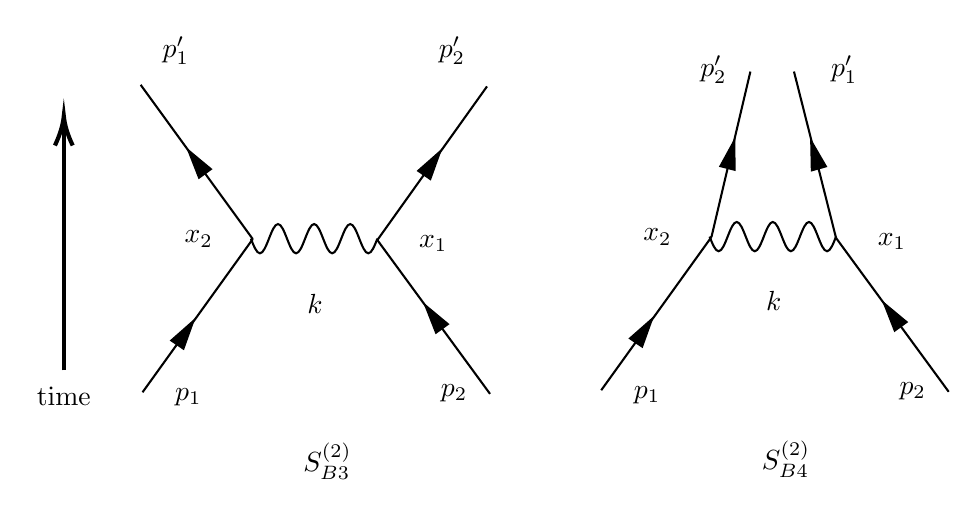
\begin{tikzpicture}[x=0.75pt,y=0.75pt,yscale=-1,xscale=1]
%uncomment if require: \path (0,300); %set diagram left start at 0, and has height of 300

%Straight Lines [id:da9046977999285625] 
\draw    (67.03,42.7) -- (121.04,117.01) ;
%Straight Lines [id:da06100511569815992] 
\draw    (121.04,117.01) -- (67.93,190.83) ;
%Shape: Wave [id:dp2673899563513945] 
\draw   (120.14,116.82) .. controls (121.56,120.43) and (122.91,123.87) .. (124.49,123.87) .. controls (126.06,123.87) and (127.42,120.43) .. (128.84,116.82) .. controls (130.26,113.21) and (131.62,109.77) .. (133.19,109.77) .. controls (134.77,109.77) and (136.13,113.21) .. (137.55,116.82) .. controls (138.97,120.43) and (140.32,123.87) .. (141.9,123.87) .. controls (143.47,123.87) and (144.83,120.43) .. (146.25,116.82) .. controls (147.67,113.21) and (149.03,109.77) .. (150.6,109.77) .. controls (152.18,109.77) and (153.54,113.21) .. (154.96,116.82) .. controls (156.38,120.43) and (157.73,123.87) .. (159.31,123.87) .. controls (160.88,123.87) and (162.24,120.43) .. (163.66,116.82) .. controls (165.08,113.21) and (166.44,109.77) .. (168.01,109.77) .. controls (169.59,109.77) and (170.95,113.21) .. (172.37,116.82) .. controls (173.79,120.43) and (175.14,123.87) .. (176.72,123.87) .. controls (178.3,123.87) and (179.65,120.43) .. (181.07,116.82) ;
%Straight Lines [id:da6329057798671613] 
\draw    (235.35,191.59) -- (181.07,117.48) ;
%Straight Lines [id:da680948881222658] 
\draw    (181.07,117.48) -- (233.9,43.46) ;
%Straight Lines [id:da4348608997197827] 
\draw [line width=1.5]    (30,180.27) -- (30,60.7) ;
\draw [shift={(30,57.7)}, rotate = 450] [color={rgb, 255:red, 0; green, 0; blue, 0 }  ][line width=1.5]    (14.21,-4.28) .. controls (9.04,-1.82) and (4.3,-0.39) .. (0,0) .. controls (4.3,0.39) and (9.04,1.82) .. (14.21,4.28)   ;
%Shape: Triangle [id:dp7748544979530381] 
\draw  [fill={rgb, 255:red, 0; green, 0; blue, 0 }  ,fill opacity=1 ] (92.34,156.6) -- (87.62,169.79) -- (81.83,165.86) -- cycle ;
%Shape: Triangle [id:dp6024942312731019] 
\draw  [fill={rgb, 255:red, 0; green, 0; blue, 0 }  ,fill opacity=1 ] (211.29,74.86) -- (206.57,88.05) -- (200.78,84.12) -- cycle ;
%Shape: Triangle [id:dp7430747380130274] 
\draw  [fill={rgb, 255:red, 0; green, 0; blue, 0 }  ,fill opacity=1 ] (204.24,149.03) -- (215.02,157.98) -- (209.35,162.08) -- cycle ;
%Shape: Triangle [id:dp5887628847311597] 
\draw  [fill={rgb, 255:red, 0; green, 0; blue, 0 }  ,fill opacity=1 ] (90.06,74.35) -- (100.84,83.3) -- (95.17,87.4) -- cycle ;
%Straight Lines [id:da9758876191029576] 
\draw    (360.8,36.3) -- (342.04,116.01) ;
%Straight Lines [id:da14762447663048084] 
\draw    (342.04,116.01) -- (288.93,189.83) ;
%Shape: Wave [id:dp35880322334435466] 
\draw   (341.14,115.82) .. controls (342.56,119.43) and (343.91,122.87) .. (345.49,122.87) .. controls (347.06,122.87) and (348.42,119.43) .. (349.84,115.82) .. controls (351.26,112.21) and (352.62,108.77) .. (354.19,108.77) .. controls (355.77,108.77) and (357.13,112.21) .. (358.55,115.82) .. controls (359.97,119.43) and (361.32,122.87) .. (362.9,122.87) .. controls (364.47,122.87) and (365.83,119.43) .. (367.25,115.82) .. controls (368.67,112.21) and (370.03,108.77) .. (371.6,108.77) .. controls (373.18,108.77) and (374.54,112.21) .. (375.96,115.82) .. controls (377.38,119.43) and (378.73,122.87) .. (380.31,122.87) .. controls (381.88,122.87) and (383.24,119.43) .. (384.66,115.82) .. controls (386.08,112.21) and (387.44,108.77) .. (389.01,108.77) .. controls (390.59,108.77) and (391.95,112.21) .. (393.37,115.82) .. controls (394.79,119.43) and (396.14,122.87) .. (397.72,122.87) .. controls (399.3,122.87) and (400.65,119.43) .. (402.07,115.82) ;
%Straight Lines [id:da07517307957898689] 
\draw    (456.35,190.59) -- (402.07,116.48) ;
%Straight Lines [id:da31330503553681854] 
\draw    (402.07,116.48) -- (381.8,36.3) ;
%Shape: Triangle [id:dp7411050182023194] 
\draw  [fill={rgb, 255:red, 0; green, 0; blue, 0 }  ,fill opacity=1 ] (313.34,155.6) -- (308.62,168.79) -- (302.83,164.86) -- cycle ;
%Shape: Triangle [id:dp81021383639529] 
\draw  [fill={rgb, 255:red, 0; green, 0; blue, 0 }  ,fill opacity=1 ] (390.1,69.86) -- (397.14,81.97) -- (390.4,83.87) -- cycle ;
%Shape: Triangle [id:dp5708438164475254] 
\draw  [fill={rgb, 255:red, 0; green, 0; blue, 0 }  ,fill opacity=1 ] (425.24,148.03) -- (436.02,156.98) -- (430.35,161.08) -- cycle ;
%Shape: Triangle [id:dp5376275039059243] 
\draw  [fill={rgb, 255:red, 0; green, 0; blue, 0 }  ,fill opacity=1 ] (353.09,69.58) -- (353.14,83.59) -- (346.36,81.87) -- cycle ;

% Text Node
\draw (90,193.27) node    {$p_{1}$};
% Text Node
\draw (218,191.27) node    {$p_{2}$};
% Text Node
\draw (84,26.27) node    {$p^{\prime }_{1}$};
% Text Node
\draw (217,26.27) node    {$p^{\prime }_{2}$};
% Text Node
\draw (95,117) node    {$x_{2}$};
% Text Node
\draw (208,119) node    {$x_{1}$};
% Text Node
\draw (151,148) node    {$k$};
% Text Node
\draw (157,224) node    {$S^{( 2)}_{B3}$};
% Text Node
\draw (311,192.27) node    {$p_{1}$};
% Text Node
\draw (439,190.27) node    {$p_{2}$};
% Text Node
\draw (343,35.27) node    {$p^{\prime }_{2}$};
% Text Node
\draw (406,35.27) node    {$p^{\prime }_{1}$};
% Text Node
\draw (316,116) node    {$x_{2}$};
% Text Node
\draw (429,118) node    {$x_{1}$};
% Text Node
\draw (372,147) node    {$k$};
% Text Node
\draw (378,223) node    {$S^{( 2)}_{B4}$};
% Text Node
\draw (30,192.87) node   [align=left] {time};


\end{tikzpicture}

    \caption{Moller Scattering}
    \label{fig:moller-scattering}
\end{figure}
In finding the result, take care to note that either $x_{1}$ or $x_{2}$ can occur first and this is already accounted for in the Dyson time ordering converted, via Wick's theorem, to normal ordering.

A separate issue is that in our expression for the transition amplitude, \textbf{the $p_{2}$ electron could be destroyed at $x_{2}$ instead of $x_{1}$ (and vice versa for the $p_{1}$ electron).} If you work the math you will see these are two different terms, each of which contributes to the amplitude. However, they have the same form if we simply switch dummy integration variables $x_{2} \leftrightarrow x_{1}$ in one of them. Hence, we will get two equal terms for the LHS of Fig. \ref{fig:moller-scattering} and two equal terms for the RHS. This allow us to use only one of them for the LHS and one for the RHS, but multiply the transition amplitude expression by 2. The final results are
\begin{equation}
\left.S_{M o l l e r}=\left(\prod_{\mathbf{p}}^{\text {all fermions}}\right) \sqrt{\frac{m}{V E_{p}}}\right)(2 \pi)^{4} \delta^{(4)}\left(p_{1}^{\prime}+p_{2}^{\prime}-p_{1}-p_{2}\right)\left(\mathcal{M}_{B 3}^{(2)}+\mathcal{M}_{B 4}^{(2)}\right)
\end{equation}
\begin{equation}
\begin{aligned}
&\mathcal{M}_{B 3}^{(2)}=+e^{2} \bar{u}_{r_1^{\prime}}\left(\mathbf{p}_{1}^{\prime}\right) \gamma^{\mu} u_{r_1}\left(\mathbf{p}_{1}\right) i D_{F \mu \nu}\left(k=p_{1}-p_{1}^{\prime}\right) \bar{u}_{r_{2}^{\prime}}\left(\mathbf{p}_{2}^{\prime}\right) \gamma^{\nu} u_{r_{2}}\left(\mathbf{p}_{2}\right)\\
&\mathcal{M}_{B 4}^{(2)}=-e^{2} \bar{u}_{r_{2}^{\prime}}\left(\mathbf{p}_{2}^{\prime}\right) \gamma^{\mu} u_{r_{1}}\left(\mathbf{p}_{1}\right) i D_{F \mu \nu}\left(k=p_{1}-p_{2}^{\prime}\right) \bar{u}_{r_{1}^{\prime}}\left(\mathbf{p}_{1}^{\prime}\right) \gamma^{v} u_{r_{2}}\left(\mathbf{p}_{2}\right)
\end{aligned}
\end{equation}
In the process of finding $\mathcal{M}_{B 3}^{(2)},$ we have to normal order. In so doing, we put the destruction operators $\psi^{+}\left(p_{1}\right)$ and $\psi^{+}\left(\mathbf{p}_{2}\right)$ at the end. But they could be ordered there as $\psi^{+}\left(p_{1}\right) \psi^{+}\left(p_{2}\right),$ or as $\psi^{+}\left(p_{2}\right) \psi^{+}\left(p_{1}\right) .$ Either would be correct normal order, but the sign of the resulting amplitude would be different. \redp{\textbf{The key is that in finding $\mathcal{M}_{B 4}^{(2)},$ we have to normal order in the same order as we did for. $\mathcal{M}_{B 3}^{(2)}$}}.

\subsection{The Electron/Positron Closed Loop Term \texorpdfstring{$S_D^{(2)}$}{TEXT}}
For the closed loop terms, we have
\begin{equation}
S_{D}^{(2)}=-\frac{1}{2 !} e^{2} \iint d^{4} x_{1} d^{4} x_{2}(N \left\{\linktwotermsl{\bar{\psi}}{\linktwoterms{\cancel{A}}{ \psi)_{x_{1}}(\bar{\psi}}{\cancel{A}} }{\psi})_{x_{2}}\right\}+N\left\{(\bar{\psi} \linktwotermsl{\cancel{A}}{ \linktwoterms{\psi}{)_{x_{1}}(}{\bar{\psi}}}{ \cancel{A}} \psi)_{x_{2}}\right\})
\label{electron-close-loop}
\end{equation}
In the manner detailed in the Box above, we can reorder either of these by switching adjacent fields (and introducing a minus sign each time we switch fermions). Doing this to the first term makes it look like the second term. Thus, (\ref{electron-close-loop}) becomes
\begin{equation}
S_{D}^{(2)}=-e^{2} \iint d^{4} x_{1} d^{4} x_{2}N\left\{(\bar{\psi} \linktwotermsl{\cancel{A}}{ \linktwoterms{\psi}{)_{x_{1}}(}{\bar{\psi}}}{ \cancel{A}} \psi)_{x_{2}}\right\}
\label{electron-close-loop2}
\end{equation}
which is represented by the following Feynman diagram
\begin{figure}[H]
    \centering
\tikzset{every picture/.style={line width=0.75pt}} %set default line width to 0.75pt        
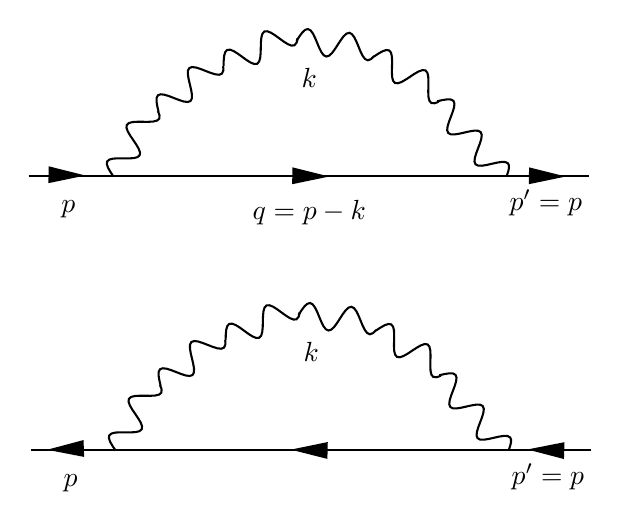
\begin{tikzpicture}[x=0.75pt,y=0.75pt,yscale=-1,xscale=1]
%uncomment if require: \path (0,300); %set diagram left start at 0, and has height of 300

%Straight Lines [id:da3309419816061372] 
\draw    (55.87,111.2) -- (325.87,111.2) ;
%Shape: Wave [id:dp1690099098873552] 
\draw   (96.77,111.45) .. controls (94.75,108.52) and (92.83,105.72) .. (93.68,104.12) .. controls (94.54,102.53) and (97.94,102.58) .. (101.5,102.64) .. controls (105.07,102.7) and (108.46,102.76) .. (109.32,101.16) .. controls (110.18,99.57) and (108.25,96.77) .. (106.23,93.83) .. controls (104.2,90.89) and (102.28,88.09) .. (103.14,86.5) .. controls (103.99,84.9) and (107.39,84.96) .. (110.96,85.02) .. controls (114.52,85.08) and (117.92,85.13) .. (118.77,83.54) .. controls (119.25,82.64) and (118.86,81.37) .. (118.06,79.9) ;
%Shape: Wave [id:dp6849760876199679] 
\draw   (118.44,80.2) .. controls (117.59,76.73) and (116.78,73.43) .. (118.15,72.24) .. controls (119.51,71.06) and (122.67,72.31) .. (125.98,73.63) .. controls (129.3,74.95) and (132.45,76.21) .. (133.82,75.02) .. controls (135.18,73.83) and (134.38,70.53) .. (133.53,67.07) .. controls (132.68,63.61) and (131.87,60.31) .. (133.24,59.12) .. controls (134.6,57.93) and (137.76,59.18) .. (141.07,60.51) .. controls (144.39,61.83) and (147.54,63.08) .. (148.91,61.89) .. controls (149.68,61.23) and (149.76,59.9) .. (149.53,58.24) ;
%Shape: Wave [id:dp4145403198216897] 
\draw   (149.75,58.16) .. controls (149.81,54.6) and (149.87,51.2) .. (151.49,50.4) .. controls (153.11,49.59) and (155.85,51.61) .. (158.72,53.73) .. controls (161.58,55.85) and (164.32,57.86) .. (165.94,57.06) .. controls (167.56,56.26) and (167.62,52.86) .. (167.68,49.3) .. controls (167.74,45.73) and (167.8,42.33) .. (169.42,41.53) .. controls (171.04,40.73) and (173.78,42.74) .. (176.64,44.86) .. controls (179.51,46.98) and (182.25,49) .. (183.87,48.2) .. controls (184.78,47.75) and (185.2,46.48) .. (185.4,44.82) ;
%Shape: Wave [id:dp37643260046922233] 
\draw   (184.87,46.06) .. controls (186.78,43.05) and (188.61,40.18) .. (190.41,40.34) .. controls (192.21,40.51) and (193.49,43.66) .. (194.83,46.96) .. controls (196.16,50.27) and (197.45,53.41) .. (199.25,53.58) .. controls (201.05,53.74) and (202.88,50.88) .. (204.79,47.87) .. controls (206.7,44.86) and (208.52,41.99) .. (210.33,42.15) .. controls (212.13,42.32) and (213.41,45.46) .. (214.75,48.77) .. controls (216.08,52.08) and (217.36,55.22) .. (219.17,55.39) .. controls (220.18,55.48) and (221.2,54.62) .. (222.23,53.31) ;
%Shape: Wave [id:dp9599988483851968] 
\draw   (222.15,53.63) .. controls (225.11,51.64) and (227.93,49.75) .. (229.51,50.62) .. controls (231.1,51.49) and (231.01,54.89) .. (230.9,58.45) .. controls (230.8,62.02) and (230.71,65.42) .. (232.29,66.29) .. controls (233.88,67.16) and (236.7,65.27) .. (239.66,63.28) .. controls (242.62,61.3) and (245.44,59.41) .. (247.03,60.28) .. controls (248.61,61.15) and (248.52,64.55) .. (248.41,68.11) .. controls (248.31,71.68) and (248.22,75.08) .. (249.8,75.95) .. controls (250.69,76.44) and (251.97,76.06) .. (253.45,75.28) ;
%Shape: Wave [id:dp887728068451431] 
\draw   (252.66,75.14) .. controls (256.07,74.33) and (259.31,73.57) .. (260.5,74.93) .. controls (261.69,76.29) and (260.5,79.41) .. (259.24,82.67) .. controls (257.98,85.93) and (256.78,89.05) .. (257.97,90.41) .. controls (259.16,91.77) and (262.41,91.01) .. (265.81,90.2) .. controls (269.22,89.4) and (272.46,88.64) .. (273.65,90) .. controls (274.84,91.36) and (273.65,94.48) .. (272.39,97.74) .. controls (271.13,101) and (269.93,104.12) .. (271.12,105.48) .. controls (272.31,106.84) and (275.56,106.08) .. (278.96,105.27) .. controls (282.37,104.47) and (285.61,103.71) .. (286.8,105.07) .. controls (287.75,106.16) and (287.18,108.37) .. (286.26,110.89) ;
%Shape: Triangle [id:dp7611450922119929] 
\draw  [fill={rgb, 255:red, 0; green, 0; blue, 0 }  ,fill opacity=1 ] (80.93,110.85) -- (65.86,113.98) -- (66.01,107.11) -- cycle ;
%Shape: Triangle [id:dp16707753725067276] 
\draw  [fill={rgb, 255:red, 0; green, 0; blue, 0 }  ,fill opacity=1 ] (198.37,111.35) -- (183.3,114.48) -- (183.44,107.61) -- cycle ;
%Shape: Triangle [id:dp18464177276205462] 
\draw  [fill={rgb, 255:red, 0; green, 0; blue, 0 }  ,fill opacity=1 ] (312.37,111.35) -- (297.3,114.48) -- (297.44,107.61) -- cycle ;
%Straight Lines [id:da2482645667024742] 
\draw    (56.87,243.2) -- (326.87,243.2) ;
%Shape: Wave [id:dp7204922677035164] 
\draw   (97.77,243.45) .. controls (95.75,240.52) and (93.83,237.72) .. (94.68,236.12) .. controls (95.54,234.53) and (98.94,234.58) .. (102.5,234.64) .. controls (106.07,234.7) and (109.46,234.76) .. (110.32,233.16) .. controls (111.18,231.57) and (109.25,228.77) .. (107.23,225.83) .. controls (105.2,222.89) and (103.28,220.09) .. (104.14,218.5) .. controls (104.99,216.9) and (108.39,216.96) .. (111.96,217.02) .. controls (115.52,217.08) and (118.92,217.13) .. (119.77,215.54) .. controls (120.25,214.64) and (119.86,213.37) .. (119.06,211.9) ;
%Shape: Wave [id:dp3337602221620415] 
\draw   (119.44,212.2) .. controls (118.59,208.73) and (117.78,205.43) .. (119.15,204.24) .. controls (120.51,203.06) and (123.67,204.31) .. (126.98,205.63) .. controls (130.3,206.95) and (133.45,208.21) .. (134.82,207.02) .. controls (136.18,205.83) and (135.38,202.53) .. (134.53,199.07) .. controls (133.68,195.61) and (132.87,192.31) .. (134.24,191.12) .. controls (135.6,189.93) and (138.76,191.18) .. (142.07,192.51) .. controls (145.39,193.83) and (148.54,195.08) .. (149.91,193.89) .. controls (150.68,193.23) and (150.76,191.9) .. (150.53,190.24) ;
%Shape: Wave [id:dp4347619235507304] 
\draw   (150.75,190.16) .. controls (150.81,186.6) and (150.87,183.2) .. (152.49,182.4) .. controls (154.11,181.59) and (156.85,183.61) .. (159.72,185.73) .. controls (162.58,187.85) and (165.32,189.86) .. (166.94,189.06) .. controls (168.56,188.26) and (168.62,184.86) .. (168.68,181.3) .. controls (168.74,177.73) and (168.8,174.33) .. (170.42,173.53) .. controls (172.04,172.73) and (174.78,174.74) .. (177.64,176.86) .. controls (180.51,178.98) and (183.25,181) .. (184.87,180.2) .. controls (185.78,179.75) and (186.2,178.48) .. (186.4,176.82) ;
%Shape: Wave [id:dp18507857213489687] 
\draw   (185.87,178.06) .. controls (187.78,175.05) and (189.61,172.18) .. (191.41,172.34) .. controls (193.21,172.51) and (194.49,175.66) .. (195.83,178.96) .. controls (197.16,182.27) and (198.45,185.41) .. (200.25,185.58) .. controls (202.05,185.74) and (203.88,182.88) .. (205.79,179.87) .. controls (207.7,176.86) and (209.52,173.99) .. (211.33,174.15) .. controls (213.13,174.32) and (214.41,177.46) .. (215.75,180.77) .. controls (217.08,184.08) and (218.36,187.22) .. (220.17,187.39) .. controls (221.18,187.48) and (222.2,186.62) .. (223.23,185.31) ;
%Shape: Wave [id:dp02539109071774759] 
\draw   (223.15,185.63) .. controls (226.11,183.64) and (228.93,181.75) .. (230.51,182.62) .. controls (232.1,183.49) and (232.01,186.89) .. (231.9,190.45) .. controls (231.8,194.02) and (231.71,197.42) .. (233.29,198.29) .. controls (234.88,199.16) and (237.7,197.27) .. (240.66,195.28) .. controls (243.62,193.3) and (246.44,191.41) .. (248.03,192.28) .. controls (249.61,193.15) and (249.52,196.55) .. (249.41,200.11) .. controls (249.31,203.68) and (249.22,207.08) .. (250.8,207.95) .. controls (251.69,208.44) and (252.97,208.06) .. (254.45,207.28) ;
%Shape: Wave [id:dp4254288717826974] 
\draw   (253.66,207.14) .. controls (257.07,206.33) and (260.31,205.57) .. (261.5,206.93) .. controls (262.69,208.29) and (261.5,211.41) .. (260.24,214.67) .. controls (258.98,217.93) and (257.78,221.05) .. (258.97,222.41) .. controls (260.16,223.77) and (263.41,223.01) .. (266.81,222.2) .. controls (270.22,221.4) and (273.46,220.64) .. (274.65,222) .. controls (275.84,223.36) and (274.65,226.48) .. (273.39,229.74) .. controls (272.13,233) and (270.93,236.12) .. (272.12,237.48) .. controls (273.31,238.84) and (276.56,238.08) .. (279.96,237.27) .. controls (283.37,236.47) and (286.61,235.71) .. (287.8,237.07) .. controls (288.75,238.16) and (288.18,240.37) .. (287.26,242.89) ;
%Shape: Triangle [id:dp2499057150249553] 
\draw  [fill={rgb, 255:red, 0; green, 0; blue, 0 }  ,fill opacity=1 ] (66.94,242.96) -- (81.81,239.01) -- (82.05,245.87) -- cycle ;
%Shape: Triangle [id:dp7780285755044771] 
\draw  [fill={rgb, 255:red, 0; green, 0; blue, 0 }  ,fill opacity=1 ] (184.37,243.03) -- (199.44,239.94) -- (199.29,246.8) -- cycle ;
%Shape: Triangle [id:dp6157200253057087] 
\draw  [fill={rgb, 255:red, 0; green, 0; blue, 0 }  ,fill opacity=1 ] (298.37,242.97) -- (313.47,240) -- (313.26,246.86) -- cycle ;

% Text Node
\draw (191,64) node    {$k$};
% Text Node
\draw (305,124) node    {$p^{\prime } =p$};
% Text Node
\draw (75,127) node    {$p$};
% Text Node
\draw (191,129) node    {$q=p-k$};
% Text Node
\draw (192,196) node    {$k$};
% Text Node
\draw (306,256) node  [rotate=-359.69]  {$p^{\prime } =p$};
% Text Node
\draw (76,259) node    {$p$};


\end{tikzpicture}
    \caption{Electron Closed Loop(top) and Positron Closed Loop(bottom)}
    \label{fig:electron-positron-closed-loop}
\end{figure}
\textbf{The dosed loop diagrams are also called self-energy diagrams.} In Fig.\ref{fig:electron-positron-closed-loop}, with closed loops, however, one of the virtual particles' 4-momentum can be anything. That is, for any value of $k$(the virtual photon 4-momentum),$q$ simply takes on the value $q=p-k$. The sum total of $k$ and $q$ must equal $p$, but this does not determine $k$ and $q$ separately. \redp{Thus, we need to integrate the expression for the transition amplitude of Fig.\ref{fig:electron-positron-closed-loop} over all values of $k$} i.e., over all values of $k^{0}$ from $-\infty$ to $+\infty$, and all yalues of $\mathbf{k}$ from $-\infty$ to $\infty$ along all three spatial directions.
$$
S_{\text {eloop}}=\left\langle e_{\mathbf{p}^{\prime}, s^{\prime}}\left|S_{D}^{(2)}\right|{e_{\mathbf{p}, s}^-}\right\rangle
$$
$$
=\left\langle e^-_{\mathbf{p}^{\prime} . s^{\prime}}\left|-e^{2} \iint d^{4} x_{1} d^{4} x_{2} i D_{F \mu \nu}\left(x_{1}-x_{2}\right)(\bar{\psi}^-)_{x_{1}} \gamma^{\mu} i S_{F}\left(x_{1}-x_{2}\right) \gamma^{\nu}\left(\psi^{+}\right)_{x_{2}}\right| e_{\mathbf{p} . s}^{-}\right\rangle
$$
$$
=-e^{2}\left\langle e_{p^{\prime}, s}^{-}\right| \iint d^{4} x_{1} d^{4} x_{2} i D_{F \mu \nu}\left(x_{1}-x_{2}\right)\left(\sum_{\mathbf{p}^{\prime}, s^{\prime\prime}} \sqrt{\frac{m}{V E_{p^{\prime \prime}}} \bar{u}_{s^{\prime\prime}}}\left(\mathbf{p}^{\prime \prime}\right) c_{s^{\prime\prime}}^{\dagger}\left(\mathbf{p}^{\prime\prime}\right) e^{i p^{\prime\prime} x_{1}}\right) \gamma^{\mu} \times
$$
$$
i S_{F}\left(x_{1}-x_{2}\right) \gamma^{\nu} \sqrt{\frac{m}{V E_{p}}} u_{s}(\mathbf{p}) e^{-i p x_{2}}|0\rangle
$$
Re-arranging factors, \textbf{\bluep{and integrate over spatial coordinates, we have}}
$$
S_{\text {e loop }}=-e^{2} \iint d^{4} q d^{4} k\left(\frac{1}{(2 \pi)^{4}}\right) \underbrace{\left(\frac{-i g_{\mu \nu}}{k^{2}+i \varepsilon}\right)}_{i D_{\mu \nu}(k)}\underbrace{\left(\int e^{-i kx_{1}} e^{-i q x_{1}} e^{i p_{1}^{\prime}x_1} d^{4} x_{1}\right)}_{(2 \pi)^{4} \delta^{(4)}\left(q-\left(p^{\prime}-k\right)\right)}\underbrace{\left(\int e^{i k x_{2}} e^{i q x_{2}} e^{-i p x_{2}} d^{4} x_{2}\right)}_{(2 \pi)^{4} \delta^{(4)}(q-(p-k))}\times
$$
$$
\frac{m}{V} \sqrt{\frac{1}{E_{p^{\prime}} E_{p}}} \bar{u}_{s^{\prime}}\left(\mathbf{p}^{\prime}\right) \gamma^{\mu} \frac{1}{(2 \pi)^{4}} \underbrace{i\left(\frac{(\not q+m)}{q^{2}-m^{2}+i \varepsilon}\right)}_{i S_{F}(q)} \gamma^{\nu} u_{s}(\mathbf{p})
$$
With the Dirac delta functions, integration over $q$ leaves $p^{\prime}-k=p-k$, meaning $p^{\prime}=p$, and thus,
$$
S_{e l o o p}=-e^{2} \delta^{(4)}\left(p-p^{\prime}=0\right) \frac{m}{V E_{p}} \int d^{4} k i D_{F \mu \nu}(k) \bar{u}_{s^{\prime}}(p) \gamma^{\mu} i S_{F}(p-k) \gamma^{\nu} u_{s}(p)
$$
We can show that only the $s=s^{\prime}$ spin state survives. Thus, the electron loop transition amplitude is
\begin{qt}
    \begin{equation}
S_{e l o o p}=\prod_{\mathbf{p}^{\prime}}^{\text {all fermions }} \sqrt{\frac{m}{V E_{p^{\prime}}}}(2 \pi)^{4} \delta^{(4)}\left(p-p^{\prime}\right) \mathcal{M}_{e l o o p}
\end{equation}
where
\begin{equation}
\mathcal{M}_{e l o o p}=\frac{-e^{2}}{(2 \pi)^{4}} \int d^{4} k i D_{F \mu \nu}(k) \bar{u}_{s}(\mathbf{p}) \gamma^{\mu} i S_{F}(p-k) \gamma^{\nu} u_{s}(\mathbf{p})
\end{equation}
\end{qt}

\subsection{The Photon Closed Loop Term \texorpdfstring{$S_E^{(2)}$}{TEXT}}
Like the electron, the photon has a closed loop interaction:
\begin{equation}
S_{E}^{(2)}=-\frac{1}{2 !} e^{2} \iint d^{4} x_{1} d^{4} x_{2} N \left\{(\linktwotermsl{\bar{\psi}}{ \cancel{A} \linktwoterms{\psi}{)_{x_{1}}(}{\bar{\psi}} \cancel{A}}{ \psi})_{x_{2}}\right\}
\label{photon-closed-loop}
\end{equation}
As presented by the Feynman diagram of Fig.\ref{fig:photon-closed-loop}, the photon closed loop (or self-energy) diagram is also known as a \redp{vacuum polarization loop} diagram because, in it, the chargeless photon sitting in the vacuum is polarized, i.e., it split into a particle with plus(pole) charge and a particle with negative (pole) charge.
\begin{figure}[H]
    \centering

\tikzset{every picture/.style={line width=0.75pt}} %set default line width to 0.75pt        

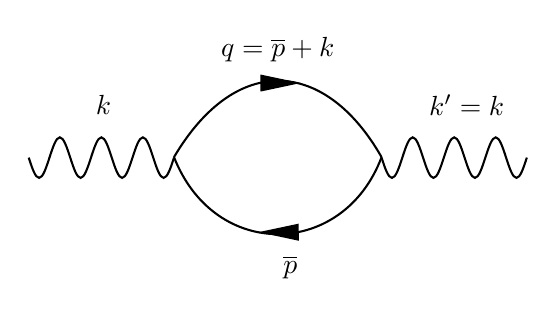
\begin{tikzpicture}[x=0.75pt,y=0.75pt,yscale=-1,xscale=1]
%uncomment if require: \path (0,300); %set diagram left start at 0, and has height of 300

%Shape: Wave [id:dp03799766308452357] 
\draw   (69,148.23) .. controls (70.63,153.24) and (72.19,158) .. (74,158) .. controls (75.81,158) and (77.37,153.24) .. (79,148.23) .. controls (80.63,143.23) and (82.19,138.47) .. (84,138.47) .. controls (85.81,138.47) and (87.37,143.23) .. (89,148.23) .. controls (90.63,153.24) and (92.19,158) .. (94,158) .. controls (95.81,158) and (97.37,153.24) .. (99,148.23) .. controls (100.63,143.23) and (102.19,138.47) .. (104,138.47) .. controls (105.81,138.47) and (107.37,143.23) .. (109,148.23) .. controls (110.63,153.24) and (112.19,158) .. (114,158) .. controls (115.81,158) and (117.37,153.24) .. (119,148.23) .. controls (120.63,143.23) and (122.19,138.47) .. (124,138.47) .. controls (125.81,138.47) and (127.37,143.23) .. (129,148.23) .. controls (130.63,153.24) and (132.19,158) .. (134,158) .. controls (135.81,158) and (137.37,153.24) .. (139,148.23) ;
%Curve Lines [id:da03627181894428755] 
\draw    (139,148) .. controls (168.87,97.47) and (211.87,100.47) .. (239,148) ;
%Curve Lines [id:da8952061471565331] 
\draw    (139,148) .. controls (158.87,198.47) and (220.87,196.47) .. (239,148) ;
%Shape: Wave [id:dp9595032443711723] 
\draw   (239,148.23) .. controls (240.63,153.24) and (242.19,158) .. (244,158) .. controls (245.81,158) and (247.37,153.24) .. (249,148.23) .. controls (250.63,143.23) and (252.19,138.47) .. (254,138.47) .. controls (255.81,138.47) and (257.37,143.23) .. (259,148.23) .. controls (260.63,153.24) and (262.19,158) .. (264,158) .. controls (265.81,158) and (267.37,153.24) .. (269,148.23) .. controls (270.63,143.23) and (272.19,138.47) .. (274,138.47) .. controls (275.81,138.47) and (277.37,143.23) .. (279,148.23) .. controls (280.63,153.24) and (282.19,158) .. (284,158) .. controls (285.81,158) and (287.37,153.24) .. (289,148.23) .. controls (290.63,143.23) and (292.19,138.47) .. (294,138.47) .. controls (295.81,138.47) and (297.37,143.23) .. (299,148.23) .. controls (300.63,153.24) and (302.19,158) .. (304,158) .. controls (305.81,158) and (307.37,153.24) .. (309,148.23) ;
%Shape: Triangle [id:dp9825029435409027] 
\draw  [fill={rgb, 255:red, 0; green, 0; blue, 0 }  ,fill opacity=1 ] (197.6,112.3) -- (181.17,115.81) -- (181.1,108.81) -- cycle ;
%Shape: Triangle [id:dp365323645361745] 
\draw  [fill={rgb, 255:red, 0; green, 0; blue, 0 }  ,fill opacity=1 ] (182.13,184.15) -- (198.57,180.67) -- (198.63,187.67) -- cycle ;

% Text Node
\draw (105,123) node    {$k$};
% Text Node
\draw (280,123) node    {$k^{\prime } =k$};
% Text Node
\draw (189,96) node    {$q=\overline{p} +k$};
% Text Node
\draw (195,201) node    {$\overline{p}$};


\end{tikzpicture}
    
    \caption{Photon Closed Loop}
    \label{fig:photon-closed-loop}
\end{figure}

Using the equation (\ref{contraction-spinor-field}), we can re-express (\ref{photon-closed-loop}) as
\begin{equation}
S_{E}^{(2)}=-\frac{1}{2 !} e^{2} \iint d^{4} x_{1} d^{4} x_{2}\left(-i S_{F \eta \alpha}\left(x_{2}-x_{1}\right)\right) \gamma_{\alpha \beta}^{\mu} i S_{F \beta \delta}\left(x_{1}-x_{2}\right) \gamma_{\delta \eta}^{\nu} N\left\{\left(A_{\mu}^{+}+A_{\mu}^{-}\right)_{x_{1}}\left(A_{\nu}^{+}+A_{\nu}^{-}\right)_{x_{2}}\right\}
\end{equation}
Since $x_1$ and $x_2$, $\mu$ and $\nu$ are dummy indeces, we find
$$
\underbrace{\left(A_{\mu}^{-}\right)_{x_{1}}\left(A_{v}^{-}\right)_{x_{2}}}_{\text {will go to zero }}\quad\underbrace{\left(A_{\mu}^{+}\right)_{x_{1}}\left(A_{v}^{+}\right)_{x_{2}}}_{\text {will go to zero }}
$$
and
$$
\underset{loop}{S_{\gamma}}=\left\langle\gamma_{\mathbf{k}^{\prime}, r^{\prime}}\right| e^{2} \iint d^{4} x_{1} d^{4} x_{2} i S_{F \eta \alpha}\left(x_{2}-x_{1}\right) \gamma_{\alpha \beta}^{\mu} i S_{F \beta \delta}\left(x_{1}-x_{2}\right) \gamma_{\delta \eta}^{\nu}\left(A_{\mu}^{-}\right)_{x_{1}}\left(A_{\nu}^{+}\right)_{x_{2}}
$$
$$
=\frac{-e^{2}}{2 V a_{k}} \delta^{(4)}\left(k-k^{\prime}\right) \int d^{4} \bar{p}\int d^{4} \bar{p} \underbrace{S_{F \eta \alpha}(\bar{p}) \gamma_{\alpha \beta}^{\mu} S_{F \beta \delta}(\bar{p}+k) \gamma_{\delta \eta}^{v}}_{\text {trace in spinor space of matrix, } M_{\eta \eta}^{\mu v}}\varepsilon_{\mu, r^{\prime}}(\mathbf{k}) \varepsilon_{v, r}(\mathbf{k})
$$
\begin{qt}
    \begin{equation}
\mathcal{M}_{\gamma}=\frac{-e^{2}}{(2 \pi)^{4}}\left\{\operatorname{Tr} \int d^{4} \bar{p} S_{F}(\bar{p}) \gamma^{\mu} S_{F}(\bar{p}+k) \gamma^{\nu}\right\} \varepsilon_{\mu, r^{\prime}}(\mathbf{k}) \varepsilon_{v, r}(\mathbf{k})
\end{equation}
\begin{equation}
S_{\gamma{\text { loop}}}=\left(\prod_{\mathbf{k}}^{\text {bosons }} \sqrt{\frac{1}{2 V \omega_{\mathbf{k}}}}\right)(2 \pi)^{4} \delta^{(4)}\left(k-k^{\prime}\right) M_{\gamma \text { loop }}
\end{equation}
\redp{Note the real positrons have positive momenta, as in the real world, whereas the virtual positron, for
our Feynman diagram and our math, has momentum equal to the negative of its true value.}
\end{qt}
\subsection{The Vacuum Bubble Term \texorpdfstring{$S_F^{(2)}$}{TEXT}}
\begin{equation}
The final non-zero term is
S_{F}^{(2)}=-\frac{1}{2 !} e^{2} \iint d^{4} x_{1} d^{4} x_{2}(\linktwotermsll{\bar{\psi}}{ \linktwotermsl{\cancel{A}}{ \linktwoterms{\psi}{)_{x_{1}}(}{\bar{\psi}} }{\cancel{A}} }{\psi})_{x_{2}}
\end{equation}
\begin{figure}[H]
    \centering

\tikzset{every picture/.style={line width=0.75pt}} %set default line width to 0.75pt        

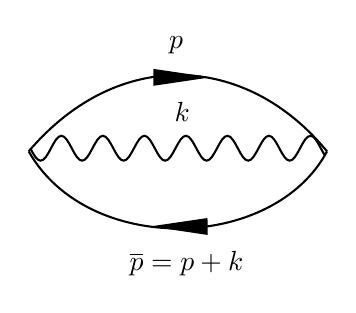
\begin{tikzpicture}[x=0.75pt,y=0.75pt,yscale=-1,xscale=1]
%uncomment if require: \path (0,300); %set diagram left start at 0, and has height of 300

%Curve Lines [id:da88424210762959] 
\draw    (391,142) .. controls (433.93,91.47) and (495.73,94.47) .. (534.73,142) ;
%Curve Lines [id:da08321555926143864] 
\draw    (391,142) .. controls (419.56,192.47) and (508.67,190.47) .. (534.73,142) ;
%Shape: Triangle [id:dp46422275430175963] 
\draw  [fill={rgb, 255:red, 0; green, 0; blue, 0 }  ,fill opacity=1 ] (475.23,106.3) -- (451.61,109.81) -- (451.51,102.81) -- cycle ;
%Shape: Triangle [id:dp600832008789588] 
\draw  [fill={rgb, 255:red, 0; green, 0; blue, 0 }  ,fill opacity=1 ] (453,178.15) -- (476.63,174.67) -- (476.7,181.67) -- cycle ;
%Shape: Wave [id:dp6468030283736343] 
\draw   (391.73,140.47) .. controls (393.36,143.54) and (394.92,146.47) .. (396.73,146.47) .. controls (398.54,146.47) and (400.1,143.54) .. (401.73,140.47) .. controls (403.36,137.39) and (404.92,134.47) .. (406.73,134.47) .. controls (408.54,134.47) and (410.1,137.39) .. (411.73,140.47) .. controls (413.36,143.54) and (414.92,146.47) .. (416.73,146.47) .. controls (418.54,146.47) and (420.1,143.54) .. (421.73,140.47) .. controls (423.36,137.39) and (424.92,134.47) .. (426.73,134.47) .. controls (428.54,134.47) and (430.1,137.39) .. (431.73,140.47) .. controls (433.36,143.54) and (434.92,146.47) .. (436.73,146.47) .. controls (438.54,146.47) and (440.1,143.54) .. (441.73,140.47) .. controls (443.36,137.39) and (444.92,134.47) .. (446.73,134.47) .. controls (448.54,134.47) and (450.1,137.39) .. (451.73,140.47) .. controls (453.36,143.54) and (454.92,146.47) .. (456.73,146.47) .. controls (458.54,146.47) and (460.1,143.54) .. (461.73,140.47) .. controls (463.36,137.39) and (464.92,134.47) .. (466.73,134.47) .. controls (468.54,134.47) and (470.1,137.39) .. (471.73,140.47) .. controls (473.36,143.54) and (474.92,146.47) .. (476.73,146.47) .. controls (478.54,146.47) and (480.1,143.54) .. (481.73,140.47) .. controls (483.36,137.39) and (484.92,134.47) .. (486.73,134.47) .. controls (488.54,134.47) and (490.1,137.39) .. (491.73,140.47) .. controls (493.36,143.54) and (494.92,146.47) .. (496.73,146.47) .. controls (498.54,146.47) and (500.1,143.54) .. (501.73,140.47) .. controls (503.36,137.39) and (504.92,134.47) .. (506.73,134.47) .. controls (508.54,134.47) and (510.1,137.39) .. (511.73,140.47) .. controls (513.36,143.54) and (514.92,146.47) .. (516.73,146.47) .. controls (518.54,146.47) and (520.1,143.54) .. (521.73,140.47) .. controls (523.36,137.39) and (524.92,134.47) .. (526.73,134.47) .. controls (528.54,134.47) and (530.1,137.39) .. (531.73,140.47) .. controls (532.4,141.73) and (533.06,142.97) .. (533.73,143.99) ;

% Text Node
\draw (467,196) node    {$\overline{p} =p+k$};
% Text Node
\draw (462,91) node    {$p$};
% Text Node
\draw (465,123) node    {$k$};


\end{tikzpicture}

    \caption{Vacuum Bubble Feynman Diagram}
    \label{fig:vacuum-bubble}
\end{figure}
\begin{qt}
    \begin{equation}
S_{F}^{(2)}=-\delta^{(4)}(0) \frac{e^{2}}{(2 \pi)^{4}} \iint S_{F \eta \alpha}(p+k) \gamma_{\alpha \beta}^{\mu} S_{F \beta \delta}(p) \gamma_{\delta \eta}^{\nu} i D_{F \mu \nu}(k) d^{4} k d^{4} p
\end{equation}
\end{qt}
In vacuum bubble means we start with zero 4-momentum in the vacuum, awe end with zero four-momentum in the vacuum, and in between we have a sum total 4 -momentum of zero for all the virtual particles mediating the interaction.

\section{Feynman Rules}
The rules themselves apply to what are termed \textbf{topologically different Feynman diagrams.} These are different from one another in ways other than simply changing labeling of vertices:
\begin{itemize}
    \item The S matrix element for a given interaction is 
    $$
S_{f i}=\delta_{f i}+\left((2 \pi)^{4} \delta^{(4)}\left(P_{f}-P_{i}\right)\right) (\prod^{\text {bosons }} \sqrt{\frac{1}{2 V \omega_{k}}})(\prod^{fermions} \sqrt{\frac{m}{V E_{\mathbf{P}}}})\mathcal{M}\quad\mathcal{M}=\sum_{n=1}^{\infty} \mathcal{M}^{(n)}
$$
where $P_{f}$ is the total 4-momentum of all final particles, $P_{i}$ is the total 4-momentum of all initial particles, and the contribution $\mathcal{M}^{(n)}$ comes from the $n$ th order perturbation term of the S operator, $S^{(n)}$
\item The Feynman amplitude $\mathcal{M}^{(n)}$ is obtained from all of the topologically distinct, connected (i.e., all lines connected to one another in a given diagram) Feynman diagrams which contain $n$ vertices. The contribution to each $\mathcal{M}^{(n)}$ is obtained by the following:

\begin{easylist}
  \ListProperties(Style1*=\bfseries,Numbers2=l,Mark1={},Mark2={)},Indent2=1em)
 @ For each vertex, include a factor $ie\gamma^{\mu}$
    
    @ For each internal photon line, labeled by 4-momentum $k$, include a factor $i D_{F \mu v}(k)=i \frac{-g_{\mu v}}{k^{2}+i \varepsilon}$
    
    @ For each internal fermion line, labeled by 4-momentum $p$, write a factor $i S_{F}(p)=i \frac{\not p+m}{p^{2}-m^{2}+i \varepsilon}$
    
    @ For each external line, write one of the following spinor factors, where $\mathbf{p}$ and $\mathbf{k}$ indicate basis states of corresponding 3 -momenta, $r$ represents spin state for fermions and polarization state for photons,
    @@ for each initial electron: $u_{r}(\mathbf{p})$
@@ for each final electron: $\bar{u}_{r}(\mathbf{p})$
@@ for each initial positron: $\bar{v}_{r}(\mathbf{p})$
@@ for each final positron: $v_{r}(\mathbf{p})$
@@ for each initial photon: $\varepsilon_{r, \mu}(\mathbf{k})$
@@ for each final photon: $\quad \varepsilon_{r, \mu}(\mathbf{k})$
@The spinor factors ( $\gamma$ matrices, $S_{F}$ functions, spinors) for each fermion line are ordered so that, reading from right to left, they occur in the same sequence as following the fermion line in the direction of its arrows through the vertex. (Order is important as it conveys spinor matrix multiplication order when we do not show spinor indices.)
@The four-momenta at each vertex are conserved (same total after as before).
@ For each closed loop of internal fermions only (without photons inside the loop itself, like what we call a "photon loop" which internally has an electron and a positron), take the trace (in spinor space) of the resulting matrix and multiply by a factor of $(-1)$
@ For each 4 -momentum $q$ which is not fixed by 4-momentum conservation, carry out the integration $\frac{1}{(2 \pi)^{4}} \int d^{4} q$ One such integration for each closed loop (fermion/fermion or fermion/photon loop).
@ Multiply the expression by (-1) for each interchange of neighboring fermion operators (each associated with a particular spinor factor) which would be required to place the expression in appropriate normal order. "Appropriate", when we are adding sub amplitudes, means each sub amplitude must be in the same, not just any, normal order of destruction and creation operators.
\end{easylist}
\end{itemize}
\begin{mybox}
Each term in $\mathcal{H}_I^I$, or equivalently in $\mathcal{L}_I^I$(since $\mathcal{L}_{I}^{I}=-\mathcal{H}_{I}^{I}$) results in a vertex interaction comprising the particles generated by the particular fields occurring in that term. Here so far, in QED, the only term in $\mathcal{L}_{I}^{I}$ is $\bar{\psi} \cancel{A} \psi$, so this gives rise to a vertex with two Dirac fermions and a photon.
\end{mybox}
\section{Including Other Charged Leptons in QED}
So far, we have dealt only with charged leptons of the electron/positron type. As physicists have learned from experiment, there are two more families of leptons, the muon/anti-muon (symbols
and $\mu^{\dagger}$ and the tau/anti-tau particle (symbols $\tau^{-}$ and $\tau^{+}$ ) families. Electrons, muons, and taus all have -1 charge. Positrons, anti-muons and anti-taus all have +1 charge. Electrons and positrons have the same mass. Muons and anti-muons have the same mass, which is about 200 times the electron mass. Taus and anti-taus have the same mass, which is about 170 times the muon mass. \textbf{The new interaction Hamiltonian that correctly describes all three families is}
\begin{equation}
\mathcal{H}_{I}^{I}=-\mathcal{L}_{I}^{I}=-e \sum_{l=1}^{3} \bar{\psi}_{l} A^{\mu} \gamma_{\mu} \psi_{l}=-e \sum_{l=1}^{3}\left(\bar{\psi}_{l}^{+}+\bar{\psi}_{l}^{-}\right)\left(\cancel{A}^{+}+\cancel{A}^{-}\right)\left(\psi_{l}^{+}+\psi_{l}^{-}\right)
\end{equation}
where the summation over $l$ represents a separate Hamiltonian density for electrons/positrons $(l=$
1), muons/anti-muons $(l=2),$ and taus/anti-taus $(l=3) .$ 
\subsection{Feynman Rules for Multiple Families}
\begin{easylist}
  @ Obtain the Feynman amplitude assuming all leptons are electrons/positrons
  @ For lines representing other lepton "flavors" replace spinor and/or propagators with those representing the other flavers.
  @ The only difference in the form of the result will be the masses.
\end{easylist}
\subsection{Elastic vs Inelastic Scattering}
The term inelastic scattering (or inelastic interaction) refers to \textbf{the particles involved changing into different types of particles with different masses (recall we mean "rest mass" by the term "mass")}, and hence some \bluep{kinetic energy must be converted into mass ( or vice versa depending on the particular interaction).}

The total amount of energy (in the form of mass plus kinetic energy) must stay the same. But if the total mass changes, then that change must be compensated for by an equivalent opposite change in kinetic energy.

Elastic scattering (or elastic interaction), on the other hand, implies we have the same type final particles (with the same masses) as the initial particles. No mass is created out of, or destroyed to yield, kinetic energy. \textbf{All energy exchange is purely kinetic, and this is a characteristic of classical elastic interactions, hence the name}.

\section{Attraction and Repulsion of Particles}
For virtual particles, \redp{3-momenturn can actually be in the opposite direction of velocity}. In fact, for attraction, this sort of behavior is essential. 3-momentum in other cases can be in other directions not parallel to virtual particle velocity (where we define that velocity in terms of the length vector between emission and absorption events divided by the time between them.)

Of course, in reality, we are looking at particles which are field-like in the sense that they are
spreading out in space. An interaction is more like an interaction of one particle field with another, and during this interaction, 3-momentum of.appropriate direction is transferred. Again, the Feynman diagrams tend to make us think of point-like particles, rather than field-like particles.

In all cases, however, we do find total 3-momentum and total energy, including all real and virtual particles, are conserved. These conservation laws still hold.

Now consider two macroscopic. charged objects approaching one another along the same line of action.When they are repulsing each other, they lose kinetic energy, and the total energy
$$
E_{\text {total}}=K E_{1}+V_{\text {classical}}+K E_{2}=\text { constant }
$$
where $V_{\text {classical}} \propto \frac{q_{1} q_{2}}{r}>0$. As their distance gets smaller, KE of the macro bodies decreases, but the electric field potential energy increases. In QFT, we would say the kinetic energies of the macro bodies plus all the energy of the virtuals is conserved,
$$
E_{\text {total}}=K E_{1}+E_{\text {virtuals}}+K E_{2}=\text { constant }
$$
And so, we can see that what is interpreted classically as classical field energy, is, in the quantum realm, energy of virtual particles,
$$
V_{\text {classical}}=E_{\text {virtuals}}>0
$$

Similar to repulsion, the classical energy relation for attraction is
$$
E_{\text {total}}=K E_{1}+V_{\text {cluascical}}+K E_{2}=const.
$$
where $V_{\text {classical}} \propto \frac{q_{1} q_{2}}{r}<0$. Given that we must have the same energy relation, in terms of virtual particles, it must mean that \textbf{the virtual particles energy must be negative as two objects approach}.
% Please add the following required packages to your document preamble:
% 
\begin{table}[H]
\caption{Summary of Virtual Photon Properties for 1D Attraction and Repulsion}
\centering
\begin{tabular}{|c|c|c|c|c|}
\hline
\multirow{2}{*}{}                                                          & \multicolumn{2}{c|}{Virtual particles in repulsion} & \multicolumn{2}{c|}{virtual particle in attraction} \\ \cline{2-5} 
                                                                           & 3-momentum                      & Energy            & 3-momentum                       & Energy           \\ \hline
\begin{tabular}[c]{@{}c@{}}Approaching and receding\\ objects\end{tabular} & $\mathbf{v}$ direction          & positive          & $-\mathbf{v}$ direction          & negative         \\ \hline
\end{tabular}
\end{table}